% (c) GreenSocs Ltd
% author: Christian Schroeder <schroeder@eis.cs.tu-bs.de>

\cleardoublepage
\chapter{GreenConfig}
\label{GreenConfig}

%%%%%%%%%%%%%%%%%%%%%%%%%%%%%%%
\section{Namespace gs::cnf and naming conventions}
The configuration specific classes of \GreenConfig have their own namespace {\sffamily gs::cnf} which is a sub namespace of the GreenSocs namespace {\sffamily gs}.

This framework uses the \GreenControl namespace {\sffamily gs::ctr}.

A \lstinline[language=TeX]|using namespace ctr;| statement in the \GreenConfig global import file imports the control namespace to the {\sffamily gs::cnf} namespace (see \Datei{greencontrol/gcnf/plugin/config\_globals.h}).

The most important classes of \GreenConfig are available within the GreenSocs namespace {\sffamily gs} as well (using statements). The classes are: \lstinline|gs_param|, \lstinline|gs_param_base| and \lstinline|gs_param_array|.

%\Note{Compatibility Note}{Namespace compativility to release 0.2}{
%	To be compatible to the old namespaces (tlm::gc, tlm::gc::config) the header
%	file \Datei{greencontrol/namespace\_compatibility.h} can be included!
%}

For the correct namespace of the classes used in this document please
refer to the doxygen generated API reference.

The classes of \GreenConfig that are visible to the user have the prefix \lstinline|GCnf|.

The \GreenConfig service, and this documentation make use of some abbreviations:
\begin{itemize}
	\item \emph{GCnf} stands for {\em GreenConfig}.
	\item \emph{cnf} or \emph{config} stand for {\em configuration}.
\end{itemize}

\paragraph{SystemC delimiter} The \GreenConfig framework is developed using the dot ({\sffamily .}) as the SystemC delimiter within names, which follows the standard. The file \Datei{gc\_globals.h} defines {\sffamily SC\_NAME\_DELIMITER} where this delimiter can be changed if the SystemC implementation e.g uses a slash ({\sffamily /}). Although this is not OSCI standard it should work for most cases.

%%%%%%%%%%%%%%%%%%%%%%%%%%%%%%%
\section{Files}
\label{GreenConfigFiles}
These are the GreenConfig files that are of interest for the user. The project can be downloaded from the GreenControl project web site (as part of the package \emph{greencontrol}).

Example files (IP, Tool,...) are located in the subdirectories of \mbox{\textsf{greencontrol/examples}}. A demonstration  platform is in the directory \mbox{\textsf{greencontrol/examples/demonstraion\_platform}}. See the \hyperlink{GCUsersGuide}{\GreenControl User's Guide} for a listing of the \GreenControl files.

Most important examples:
\begin{itemize}

  \item \Verzeichnis{greencontrol/examples/regression\_tests}: \newline
  	Different test IPs which use different parameters and a test tool which uses the \GreenConfig \lstinline|Tool_Api| to set and get parameters of the TestIP.

  \item \Verzeichnis{greencontrol/examples/demonstration\_platform}: \newline
  	Demonstration platform (testbench file \Datei{testbench\_demonstration\_platform.cpp} and configuration files \Datei{demoplatform\textless x\textgreater.cfg}.

  \item \Verzeichnis{greencontrol/examples/user\_api\_example}:  \newline
  	Example API which uses the gc\_ports directly (file \Datei{tool\_api/tool\_api.h}).

  \item \Verzeichnis{greencontrol/examples/gcnf\_private\_params}:  \newline
  	Example with private parameters and private APIs.

  \item \Verzeichnis{greencontrol/examples/parameter\_arrays}:  \newline
  	Example with Simple Parameter Arrays.

  \item \Verzeichnis{greencontrol/examples/extended\_parameter\_arrays}:  \newline
  	Example with Extended Parameter Arrays.

  \item \Verzeichnis{greencontrol/examples/callback\_example}:  \newline
  	Example showing the parameter's callback functionality.

  \item \Verzeichnis{greencontrol/gcnf/apis/commandLine\_Tool}:  \newline
  	User API adapter (class \lstinline|CommandLine_Tool|) which provides a command line inside the simulation terminal.

  \item \Verzeichnis{greencontrol/gcnf/apis/commandLineConfigParserApi}:  \newline
  	User API adapter (class \lstinline|CommandLineConfigParser|) which reads in parameters from the command line.
\end{itemize}


\noindent
\begin{minipage}{\textwidth}
\begin{tabularx}{\textwidth}{|l|X|}
	\cline{1-1}\cline{2-2}\multicolumn{2}{|l|}{  {\bf\sffamily greencontrol}    }\\
	\cline{1-1}\cline{2-2}  config.h &   Main user include file. Includes the config plugin, the standard GCnf API and the parameters.   \\
	\hline
	\cline{1-1}\cline{2-2}  config\_api\_command\_line\_parser.h &   Includes the command line parser which handles command line arguments setting parameter values.  \\
	\hline
	\cline{1-1}\cline{2-2}  config\_api\_command\_line\_tool.h &   Includes the tool which provides a command line during the simulation, allowing direct configuration and inspection during simulation runtime.  \\
	\hline
	\cline{1-1}\cline{2-2}  config\_api\_config\_file\_parser.h &   Includes the configuration file parser. \\
	\hline
	\cline{1-1}\cline{2-2}  config\_api\_lua\_file\_parser.h &   Includes the LUA configuration file parser. \\
	\hline
\end{tabularx}
\end{minipage}

\vspace{1 cm}

\noindent
\begin{minipage}{\textwidth}
\begin{tabularx}{\textwidth}{|l|X|}
	\cline{1-1}\cline{2-2}\multicolumn{2}{|l|}{  {\bf\sffamily greencontrol/docs/GreenConfig}    }\\
	\cline{1-1}\cline{2-2}  users\_guide/latex/GCnf\_Users\_Guide.pdf &            This User's Guide.  \\
	\cline{1-1}\cline{2-2}  tutorial/latex/GreenConfig\_Tutorial.pdf &                 Tutorial of use.  \\
	\cline{1-1}\cline{2-2}  api\_ref/index.html &        Link page to API Reference. \\
	%\cline{1-1}\cline{2-2}  gc\_doxygen\_brief.conf &    Doxygen configuration file for generation brief API reference. \\
	%\cline{1-1}\cline{2-2}  gc\_doxygen\_detailed.conf & Doxygen configuration file for generation detailed API reference.  \\
	%\cline{1-1}\cline{2-2}  api\_ref/brief/html/* &      Brief API Reference. \\
	%\cline{1-1}\cline{2-2}  api\_ref/detailed/html/* &   Detailed API Reference.  \\
	\hline
\end{tabularx}
\end{minipage}

\vspace{1 cm}

%\noindent
%\begin{minipage}{\textwidth}
%\begin{tabularx}{\textwidth}{|l|X|}
%	\cline{1-1}\cline{2-2}\multicolumn{2}{|l|}{  {\bf greencontrol/gcnf/plugin}    }\\
%	\cline{1-1}\cline{2-2} config\_callbadapt.h    &  \WarningSymbol {\em Deprecated} classes \lstinline|CallbAdapt_b| and templated \lstinline|CallbAdapt<...>| for providing user defined callback function pointers to the \lstinline|GCnf_Api|.   \\
%	\cline{1-1}\cline{2-2} config\_globals.h    &  Global settings for the \GreenConfig service.   \\
%	\cline{1-1}\cline{2-2} config\_paramcallbadapt.h    &  Classes \lstinline|ParamCallbAdapt_b| and templated \lstinline|ParamCallbAdapt<...>| for providing user defined callback function pointers to the parameters (\lstinline|gs_param|s).   \\
%	\cline{1-1}\cline{2-2} configdatabase.h    &  Class \lstinline|ConfigDatabase| is the standard parameter database which is used by the Config Plugin and instantiated in the top level.   \\
%	\cline{1-1}\cline{2-2} configplugin.h    &  Contains the Configuration Plugin.   \\
%	\cline{1-1}\cline{2-2} gcnf\_datatypes.h    &  Data types specific for \GreenConfig: class \lstinline|ConfigCommand| command enumeration for the transaction container. \\
%	\cline{1-1}\cline{2-2} observer\_db\_if.h &  Interface to be implemented by the observer databases and used in the SystemC port of the plugin. \\
%	\cline{1-1}\cline{2-2} observerdatabase.h    &  Standard observer database instantiated and bound in the plugin.   \\
%	\cline{1-1}\cline{2-2} param\_db\_if.h &  Interface to be implemented by the parameter databases and used in the SystemC port of the plugin. \\
%	\cline{1-1}\cline{2-2} plugin\_if.h &  Interface implemented by the plugin to allow the observer database to access special functions of the parameter database. \\
%	\hline
%\end{tabularx}
%\end{minipage}

%\vspace{1 cm}

%\noindent
%\begin{minipage}{\textwidth}
%\begin{tabularx}{\textwidth}{|l|X|}
%	\cline{1-1}\cline{2-2}\multicolumn{2}{|l|}{  {\bf greencontrol/gcnf/apis/GCnf\_Api}    }\\
%	\cline{1-1}\cline{2-2} GCnf\_Api.h    &  User inlcude file to make the Config API class available.  \\
%	\cline{1-1}\cline{2-2} GCnf\_Api\_t.h    &  Implementation of \GreenControl Config API (typedefed to class \lstinline|GCnf_Api|) can be used by the User API adapters. The \lstinline|GCnf_Api| owns the \lstinline|gc_port|.   \\
%	\cline{1-1}\cline{2-2} gcnf\_api.h    &  Config API interface \lstinline|cnf_api_if|.  \\
%	\hline
%\end{tabularx}
%\end{minipage}

%\vspace{1 cm}

%\noindent
%\begin{minipage}{\textwidth}
%\begin{tabularx}{\textwidth}{|l|X|}
%	\cline{1-1}\cline{2-2}\multicolumn{2}{|l|}{  {\bf greencontrol/gcnf/apis/GCnf\_private\_Api}    }\\
%	\cline{1-1}\cline{2-2} gcnf\_private\_api.h         &  Private Config API class.  \\
%	%\cline{1-1}\cline{2-2} gcnf\_private\_plugin.h    &  Private Config Plugin API similar to the Config Plugin.  \\
%	\hline
%\end{tabularx}
%\end{minipage}

%\vspace{1 cm}

%\noindent
%\begin{minipage}{\textwidth}
%\begin{tabularx}{\textwidth}{|l|X|}
%	\cline{1-1}\cline{2-2}\multicolumn{2}{|l|}{  {\bf greencontrol/gcnf/apis/gs\_param}    }\\
%	\cline{1-1}\cline{2-2} gs\_param\_array.h   &  Extended Parameter Arrays \\
%	\cline{1-1}\cline{2-2} gs\_param\_array.hpp   &  Simple Parameter Arrays \\
%	\cline{1-1}\cline{2-2} gs\_param\_base.h    &  Base class for template specialized objects \lstinline|gs_param_t|. Uses the \lstinline|GCnf_Api|.   \\
%	\cline{1-1}\cline{2-2} gs\_param\_native.hpp     &  Specializations of the gs\_param class for native C/C++ data types.   \\
%	\cline{1-1}\cline{2-2} gs\_param\_operator\_macros.h    &  Macros for the template specializations in \lstinline|gs_param|.   \\
%	\cline{1-1}\cline{2-2} gs\_param\_systemc.hpp    &  Specializations of the gs\_param class for SystemC data types.   \\
%	\cline{1-1}\cline{2-2} gs\_param\_t         &  Templated base class for the parameters \lstinline|gs_param|.   \\
%	\cline{1-1}\cline{2-2} gs\_param.h         &  \GreenConfig parameter objects.   \\
%	\hline
%\end{tabularx}
%\end{minipage}

%\vspace{1 cm}

\noindent
\begin{minipage}{\textwidth}
\begin{tabularx}{\textwidth}{|l|X|}
	\cline{1-1}\cline{2-2}\multicolumn{2}{|l|}{  {\bf\sffamily greencontrol/gcnf/apis/scmlApi}    }\\
	%\cline{1-1}\cline{2-2} operator\_macros.h    &  Macros for the template specializations in \lstinline|scml_property|.   \\
	%\cline{1-1}\cline{2-2} scml\_api.h    &  User API adapter class \lstinline|Scml_Api| which connects to a \lstinline|GCnf_Api| and translates between \lstinline|scml_property| objects and the \lstinline|GCnf_Api|.   \\
	\cline{1-1}\cline{2-2} scml\_property.h    &  Objects which can be used as parameters in the user code. All objects of one module use together one instance of the \lstinline|Scml_Api|.    \\
	%\cline{1-1}\cline{2-2} scml\_property.tpp    &  Implementations for the class \lstinline|gcnfScmlProperty_base|.    \\
	\hline
\end{tabularx}
\end{minipage}

\vspace{1 cm}

%\noindent
%\begin{minipage}{\textwidth}
%\begin{tabularx}{\textwidth}{|l|X|}
%	\cline{1-1}\cline{2-2}\multicolumn{2}{|l|}{  {\bf greencontrol/gcnf/apis/configFileApi}    }\\
%	\cline{1-1}\cline{2-2} configfile\_tool.h     &  Class \lstinline|ConfigFile_Tool| to read a configuration file and configure the parameters.   \\
%	%\cline{1-1}\cline{2-2} gc\_config\_parser.h    &  Methods which are used by the \lstinline|ConfigFile_Tool|.   \\
%	\hline
%\end{tabularx}
%\end{minipage}

%\vspace{1 cm}

\noindent
\begin{minipage}{\textwidth}
\begin{tabularx}{\textwidth}{|l|X|}
	\cline{1-1}\cline{2-2}\multicolumn{2}{|l|}{  {\bf\sffamily greencontrol/gcnf/apis/toolApi}    }\\
	\cline{1-1}\cline{2-2} tool\_gcnf\_api.h    &  User API adapter class \lstinline|Tool_GCnf_Api| for initial and runtime configuration which uses the \lstinline|GCnf_Api|.   \\
	\hline
\end{tabularx}
\end{minipage}


%%%%%%%%%%%%%%%%%%%%%%%%%%%%%%%
\section{Quick Start}

To use \GreenConfig at least the following include is needed:
%\begin{lstlisting}
%#include "greencontrol/core/gc_core.h"  // GreenControl Core
%#include "greencontrol/gcnf/plugin/configplugin.h"   // ConfigPlugin
%#include "greencontrol/gcnf/plugin/configdatabase.h" // ConfigDatabase
%\end{lstlisting}
\begin{lstlisting}
#include "greencontrol/config.h"
\end{lstlisting}

\noindent
\begin{minipage}{\textwidth}
\paragraph{Recommended:} The {\sffamily sc\_main} should initialize the framework before instantiating any user modules:
\begin{lstlisting}
int sc_main(int argc, char *argv[]) {
  /// GreenControl Core instance
  gs::ctr::GC_Core       core;
  // GreenConfig Plugin
  gs::cnf::ConfigPlugin configPlugin;

  // User modules etc.

  sc_start();
  return EXIT_SUCCESS;
}
\end{lstlisting}
\end{minipage}

\noindent
\begin{minipage}{\textwidth}
\paragraph{Alternative} If you don't care on which classes are included, alternatively this short variant may be used, which includes and instantiates some more parts of \GreenControl and its sub-projects (e.g. \GreenConfig, \GreenAV):
\begin{lstlisting}
// Standard GreenControl with config and analysis
#include "greencontrol/all.h"

int sc_main(int argc, char *argv[]) {
  // Standard GreenControl instantiations (Core, GreenConfig, GreenAV)
  GS_INIT_STANDARD_GREENCONTROL;

  // User modules etc.

  sc_start();
  return EXIT_SUCCESS;
}
\end{lstlisting}
\end{minipage}


\begin{itemize}
  \item The include {\sffamily greencontrol/all.h} includes many useful classes of several projects. Additional linking may be needed (e.g. link to lua). This may change independently of this documentation, see the code for the currently included files.
  \item The macro {\sffamily GS\_INIT\_STANDARD\_GREENCONTROL} has to be used in the main function (or equal) and instantiates several standard elements. E.g. these are the Core, the \GreenConfig and \GreenAV plugins. This may change independently of this documentation, see the code (file \Datei{greencontrol/core/gc\_globals.h}) for the current configuration.
\end{itemize}

\noindent
\begin{minipage}{\textwidth}
\paragraph{Short (experimental):} As another alternative you can rely on the automatic creation of the \GreenControl Core and the Configuration Plugin with the default database (see section \ref{GCnfAutomaticConstruction}). In this case the {\sffamily sc\_main} needs not to initialize the framework:
\begin{lstlisting}
int sc_main(int argc, char *argv[]) {

  // User modules etc.

  sc_start();
  return EXIT_SUCCESS;
}
\end{lstlisting}
\end{minipage}


%%%%%%%%%%%%%%%%%%%%%%%%%%%%%%%
\section{Processing flow GreenControl and GreenConfig}
In this section, an example flow shows what the framework does during construction time and preparation for simulation -- if the recommended initialization style is used. Automatic instantiation differs.

%{\em initial-mode}

\begin{itemize}
	\item The GC\_Core is instantiated,

	\item The required plugins are instantiated (ConfigPlugin)
	\begin{itemize}
		\item The gc\_port searches for the global GC\_Core instance and connects automatically.
	\end{itemize}

	\item A default user config API is instantiated
	\begin{itemize}
		\item The contained gc\_port performs automatic binding to the Core.
	\end{itemize}

	\item Parameters are instantiated:
	\begin{itemize}
		\item A user API is instantiated (containing a gc\_port)
		\begin{itemize}
			\item The contained gc\_port performs automatic binding to the Core.
		\end{itemize}
	\end{itemize}
	\item Parameters are added (with default value) to the Config Plugin.

	\item Other IPs are instantiated.
	\begin{itemize}
		\item ...
	\end{itemize}

  \item Instantiate Tool API
  \begin{itemize}
		\item gc\_port bound automatically (see above)
		\item Command get (etc.) may be used
	\end{itemize}

	\item Core (CallbackDispatcher) gets SystemC kernel callback start\_of\_simulation
	\begin{itemize}
		\item Core calls start\_initial\_configuration in each API  \newline The APIs may perform further initial configuration.
		\item After that Core calls end\_initialize\_mode in each API
	\end{itemize}
\end{itemize}

%{\em runtime-mode}


%%%%%%%%%%%%%%%%%%%%%%%%%%%%%%%
\section{Configuration Service CONFIG\_SERVICE}

%%%%%
\subsection{Configuration Plugin ConfigPlugin}
\label{ConfigPlugin}

The plugin which provides the configuration service is the \lstinline|ConfigPlugin|. In its \lstinline|gc_port| the supported service is set to \lstinline|CONFIG_SERVICE| and the boolean \lstinline|is_plugin| is set to true.

The ConfigPlugin provides and uses the commands listed in the following section. Pointers to parameters are stored in a \emph{parameter database} and observer addresses are stored in a separate \emph{observer database}. Both databases have to implement interfaces (\lstinline|param_db_if| and \lstinline|observer_db_if|) and are used by the ConfigPlugin, see figure \ref{fig:ConfigPluginDatabaseConnection}.% The plugin implements the \lstinline|plugin_if| to allow the observer database to access special functions of the parameter database.

The framework stores the values of the parameters not in the database but in the parameter objects themselves. The parameter database holds 'only' pointers to the parameters. This makes access to parameters fast.

\Note{Compatibility}{\WarningSymbol{Deprecated}}{
For compatibility (to the \GreenConfig framework revision 0.2) a User API still is allowed to add new parameters by name and value, not by pointer. In this case the plugin creates a parameter object and adds that pointer to the database. All \lstinline|gs_param| usages and API method calls keep the same for compatibility. Some of the calls are deprecated due to speed reasons. When deprecated methods are called, an \textsf{SC\_WARNING} is reported (macro \textsf{DEPRECATED\_WARNING}) which can be disabled by defining \mbox{\lstinline[language=XML]|#define NO_DEPRECATED_WARNINGS|} in \Datei{greencontrol/core/gc\_globals.h} or the makefile/compiler settings.
}

%That makes accesses to the parameters much faster. Now parameters can be used during simulation more frequently

The \GreenConfig standard parameter database is the
\lstinline|ConfigDatabase|. It has to be instantiated in the top-level
(testbench) --~if not created automatically~-- and is given to the ConfigPlugin constructor. The
parameter database can be replaced by another one, e.g. an adapter to
the scml database (registry, server). Note the following design rule:

\Note{Design rule}{\WarningSymbol{Database and ConfigPlugin deletion}}{
	Create the database {\em before} the plugin and ensure that the deletion happens in reverse order!
}

The standard observer database is the \lstinline|ObserverDatabase| which stores addresses of observers that are registered to be called when a new parameter is created. The observer database is instantiated and bound in the plugin. It gets a pointer to the plugin to be able to bind the \lstinline|plugin_if| port.

The ConfigPlugin includes and construction can be done as follows:

\noindent
\begin{minipage}{\textwidth}
\begin{lstlisting}
#include "greencontrol/config.h"
// in sc_main (or elsewhere):
gc::cnf::ConfigDatabase db("CnfDb");
gc::cnf::ConfigPlugin configPlugin(&db);
\end{lstlisting}
\end{minipage}

\WarningSymbol{Warning:} Do not new the ConfigDatabase directly inside the plugin construction. With some compilers this may lead to an SystemC runtime error because of a failure in the SystemC module stack.

\noindent
\begin{minipage}{\textwidth}
Another way creating the standard configuration plugin is calling the static get function. Note that this news the config plugin one time as singleton (if not created by the user before), strictly speaking this is a memory leak if is not been deleted after simulation -- in the correct order after all APIs and parameters but before the core. This call works together with a previously manually created plugin.
\begin{lstlisting}
#include "greencontrol/config.h"
// in sc_main (or elsewhere):
gs::cnf::ConfigPlugin::get_instance();
\end{lstlisting}
\end{minipage}

\begin{figure}[htb]
	\centerline{
		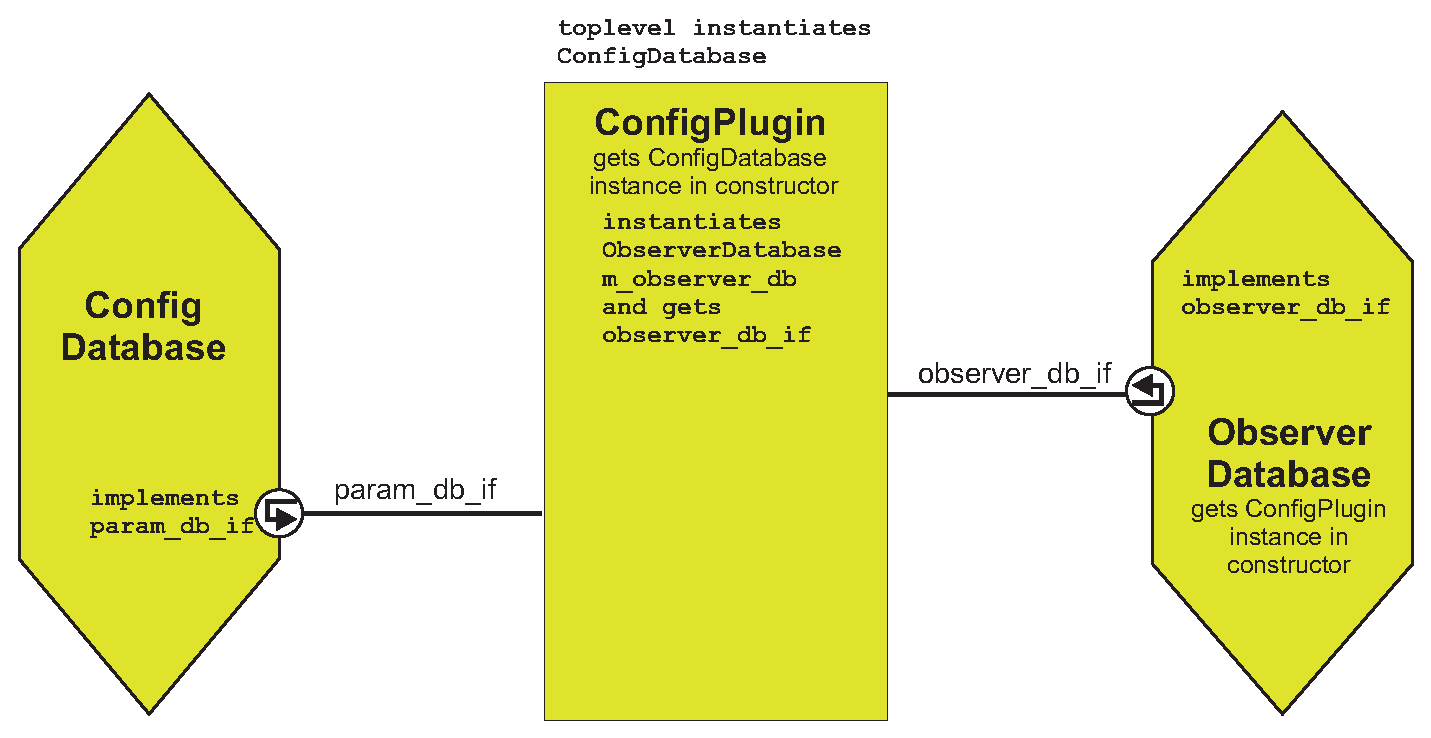
\includegraphics[width=\textwidth]{ConfigPlugin_Ports.eps}}
	\caption{Connection of databases to the configuration plugin with interfaces.}
	\label{fig:ConfigPluginDatabaseConnection}
\end{figure}


%%%%%
\subsection{Alternative automatic construction}
\label{GCnfAutomaticConstruction}

\WarningSymbol{Warning:} \textbf{This is experimental.} Please report problems to christian.schroeder@greensocs.com!

Similar to the automatic \GreenControl Core construction the configuration plugin can be automatically constructed - with its standard database.

On the first instantiation of any parameter or GCnf API the plugin will be created automatically.

\begin{itemize}
  \item The plugin will be instantiated with the standard database class \lstinline|gs::config::ConfigDatabase|.
  \item This only works if there is any instantiation of a parameter or GCnf API before the \lstinline|sc_start| call!
\end{itemize}


%%%%%
\subsection{Commands for the Configuration Service (internal)}
\label{CommandsConfigService}

In the configuration service (\lstinline|CONFIG_SERVICE|) the command enumeration \lstinline|ConfigCommand| is used. The plugin and the APIs have to know how to process each command. If a user wants to add a new command, it has to be added to the enumeration and the ConfigPlugin and the affected APIs have to be adapted. The plugin and the \lstinline|GCnf_Api|  throw a warning if the command is unknown.

All configuration command may be used during elaboration and runtime.

The following commands may be used by the Config APIs. The fields of the transaction are used for special commands on the shown way:

\ZwischenUberschrift{Direction: API $\rightarrow$ ConfigPlugin}

\noindent
\begin{tabularx}{\textwidth}{|p{3.6cm}|p{2.3cm}|p{2cm}|X|}
	\cline{1-1}\cline{2-2}\cline{3-3}\cline{4-4} Command                &  Phase       &  Field             &  Description   \\
\end{tabularx}
\begin{tabularx}{\textwidth}{|p{3.6cm}|X|}
	\cline{1-1}\cline{2-2}
	 \lstinline|CMD_ADD_PARAM| & Adds a parameter {\em and} sets its default value. This command may only be used by the parameter owning module. The default value has to be set with this command and {\em not} with a following CMD\_SET\_PARAM to allow other modules (e.g. tool, config file parser tools) to overwrite the default value.  \newline This command creates an explicit parameter or converts an implicit to an explicit by not overwriting the implicit set init value.  \\
\end{tabularx}
\begin{tabularx}{\textwidth}{|p{3.6cm}|p{2.3cm}|p{2cm}|X|}
	\cline{1-1}\cline{2-2}\cline{3-3}\cline{4-4}
	 &  REQUEST     &  {\em AnyPointer}    &  Parameter pointer.   \\
	\cline{1-1}\cline{2-2}\cline{3-3}\cline{4-4}
	                        &  REQUEST     &  alternative  \newline{\em Specifier}        &  Name of a parameter that should be created by the plugin.  \\
	\cline{4-4}                        &      &  and \newline{\em Value}        &  Value of the parameter that should be created by the plugin.  \\
	\cline{1-1}\cline{2-2}\cline{3-3}\cline{4-4}
	                        &  RESPONSE    &  {\em Error}       &  $>0$ when adding fails.   \\
	\hline
\end{tabularx}

\vspace{1 cm}

\noindent
\begin{tabularx}{\textwidth}{|p{3.6cm}|X|}
	\cline{1-1}\cline{2-2}
	  \lstinline|CMD_SET_INIT_VAL| & Sets the init value of a parameter. If the parameter does not yet exist, it is created as an implicit parameter. The init value of an implicit parameter has priority to the initial value of a new added parameter. This command overrides the default value which was/will be set during adding a parameter. This gives tools the opportunity to set initial values. See section \ref{ParameterTypesImplExpl}. \\
\end{tabularx}
\begin{tabularx}{\textwidth}{|p{3.6cm}|p{2.3cm}|p{2cm}|X|}
	\cline{1-1}\cline{2-2}\cline{3-3}\cline{4-4}
	   &  REQUEST     &  {\em Specifier}   &  Parameter name.   \\
	\cline{1-1}\cline{2-2}\cline{3-3}\cline{4-4}                        &  REQUEST     &  {\em Value}     &  Init value of the parameter.   \\
	\cline{1-1}\cline{2-2}\cline{3-3}\cline{4-4}                        &  RESPONSE    &  {\em Error}    &  No error specified so long.\\
	\hline
\end{tabularx}

\vspace{1 cm}

\noindent
\begin{tabularx}{\textwidth}{|p{3.6cm}|X|}
	\cline{1-1}\cline{2-2}
	  \lstinline[breaklines=false]|CMD_LOCK_INIT_VAL| & Locks the init value of a parameter. Lock so that this parameter's init value cannot be overwritten by  any subsequent \lstinline|CMD_SET_INIT_VAL|. This allows to emulate a hierarchical
    precendence since a top-level module can prevent the childs from setting
    init values by locking the init value before creating the subsystem.\newline   
    Returns false (and does not lock) if parameter is already existing explicitely.\newline
    Returns false (and does not lock) if no initial value is existing that can be locked. \\
\end{tabularx}
\begin{tabularx}{\textwidth}{|p{3.6cm}|p{2.3cm}|p{2cm}|X|}
	\cline{1-1}\cline{2-2}\cline{3-3}\cline{4-4}
	   &  REQUEST     &  {\em Specifier}   &  Parameter name.   \\
	\cline{1-1}\cline{2-2}\cline{3-3}\cline{4-4}                        &  RESPONSE    &  {\em Error}    &  $>0$ when parameter lock was not applied.   \\
	\hline
\end{tabularx}

\vspace{1 cm}

\noindent
\begin{tabularx}{\textwidth}{|p{3.6cm}|X|}
	\cline{1-1}\cline{2-2}
	  \lstinline|CMD_GET_VAL| & Gets the string representation of the parameter value. May be used for implicit and explicit parameters.\\
\end{tabularx}
\begin{tabularx}{\textwidth}{|p{3.6cm}|p{2.3cm}|p{2cm}|X|}
	\cline{1-1}\cline{2-2}\cline{3-3}\cline{4-4}
	  &  REQUEST     &  {\em Specifier}   &  Parameter name.   \\
	\cline{1-1}\cline{2-2}\cline{3-3}\cline{4-4}                        &  RESPONSE    &  {\em Value} &  String representation of the parameter's value.   \\
	\cline{1-1}\cline{2-2}\cline{3-3}\cline{4-4}                        &  RESPONSE    &  {\em Error}  &  $>0$ when parameter does not exist implicit or explicit.   \\
	\hline
\end{tabularx}

\vspace{1 cm}

\noindent
\begin{tabularx}{\textwidth}{|p{3.6cm}|X|}
	\cline{1-1}\cline{2-2}
	  \lstinline|CMD_GET_PARAM| & Gets a pointer to a parameter. This should not be done for a none existing parameter. (The error flag will be set in the transaction.)\\
\end{tabularx}
\begin{tabularx}{\textwidth}{|p{3.6cm}|p{2.3cm}|p{2cm}|X|}
	\cline{1-1}\cline{2-2}\cline{3-3}\cline{4-4}
	   &  REQUEST     &  {\em Specifier}   &  Parameter name.   \\
	\cline{1-1}\cline{2-2}\cline{3-3}\cline{4-4}                        &  RESPONSE    &  {\em AnyPointer} &  Pointer to the parameter.   \\
	\cline{1-1}\cline{2-2}\cline{3-3}\cline{4-4}                        &  RESPONSE    &  {\em Error}  &  $>0$ when getting fails.   \\
	\hline
\end{tabularx}

\vspace{1 cm}

\noindent
\begin{tabularx}{\textwidth}{|p{3.6cm}|X|}
	\cline{1-1}\cline{2-2}
	  \lstinline|CMD_REMOVE_PARAM| & Removes a parameter from the plugin.\\
\end{tabularx}
\begin{tabularx}{\textwidth}{|p{3.6cm}|p{2.3cm}|p{2cm}|X|}
	\cline{1-1}\cline{2-2}\cline{3-3}\cline{4-4}
	   &  REQUEST     &  {\em AnyPointer}   &  Pointer to parameter.   \\
	\cline{1-1}\cline{2-2}\cline{3-3}\cline{4-4}                        &  RESPONSE    &  {\em Error}  &  $>0$ when removement not successful. \\
	\hline
\end{tabularx}

\vspace{1 cm}

\noindent
\begin{tabularx}{\textwidth}{|p{3.6cm}|X|}
	\cline{1-1}\cline{2-2}
	  \lstinline|CMD_EXISTS_PARAM| & Returns if the parameter exists. To return true the parameter may exist as implicit or explicit parameter. \\
\end{tabularx}
\begin{tabularx}{\textwidth}{|p{3.6cm}|p{2.3cm}|p{2cm}|X|}
	\cline{1-1}\cline{2-2}\cline{3-3}\cline{4-4}
	   &  REQUEST     &  {\em Specifier}   &  Parameter name.   \\
	\cline{1-1}\cline{2-2}\cline{3-3}\cline{4-4}                        &  RESPONSE    &  {\em Error}  &  $=0$ : Parameter existing \newline $=1$ : Parameter not existing   \\
	\hline
\end{tabularx}

\vspace{1 cm}

\noindent
\begin{tabularx}{\textwidth}{|p{3.6cm}|X|}
	\cline{1-1}\cline{2-2}
	  \lstinline|CMD_GET_ PARAM_LIST_VEC| & Returns a vector of parameter names.  \newline Depends on flag mSpecifier:  \newline  empty: Gets list of all existing parameters in the plugin.  \newline  modulename (e.g. jpeg.encoder): Returns all parameters of the specified module (without its child modules).  \newline  modulename.* (e.g. jpeg.*): Returns all parameters of the specified module including the parameters of its child modules.\\
\end{tabularx}
\begin{tabularx}{\textwidth}{|p{3.6cm}|p{2.3cm}|p{2cm}|X|}
	\cline{1-1}\cline{2-2}\cline{3-3}\cline{4-4}
	   &  REQUEST     &  {\em Specifier}   &  Empty or module name or \newline\mbox{\textless modulename\textgreater.*}   \\
	\cline{1-1}\cline{2-2}\cline{3-3}\cline{4-4}                        &  RESPONSE    &  {\em AnyPointer}  & Vector of names (strings) of the requested parameters (all existing or all of that module or all of that module + childs). \newline Receiver must delete the pointer! \\
	\cline{1-1}\cline{2-2}\cline{3-3}\cline{4-4}                        &  RESPONSE    &  {\em Error}  &  No error specified so long. \\
	\hline
\end{tabularx}

\vspace{1 cm}

\noindent
\begin{tabularx}{\textwidth}{|p{4cm}|X|}
	\cline{1-1}\cline{2-2}
	  \lstinline|CMD_REGISTER_NEW_ PARAM_OBSERVER| & Registers an observer for new added or new set parameters.  \\
\end{tabularx}
\begin{tabularx}{\textwidth}{|p{4cm}|p{2.3cm}|p{2cm}|X|}
	\cline{1-1}\cline{2-2}\cline{3-3}\cline{4-4}
	 &  REQUEST     &  {\em ID}:    &  Observer's address.   \\
	\cline{1-1}\cline{2-2}\cline{3-3}\cline{4-4}                                      &  RESPONSE    &  {\em Error}:        &  $>0$ when registering failed.  \\
	\hline
\end{tabularx}

\vspace{1 cm}

\noindent
\begin{tabularx}{\textwidth}{|p{4cm}|X|}
	\cline{1-1}\cline{2-2}
	  \lstinline|CMD_UNREGISTER_ PARAM_CALLBACK| & Unregisters all parameter callbacks for the specified observer module. The callbacks were previously registered by the module directly at the parameters.\\
\end{tabularx}
\begin{tabularx}{\textwidth}{|p{4cm}|p{2.3cm}|p{2cm}|X|}
	\cline{1-1}\cline{2-2}\cline{3-3}\cline{4-4}
	 &  REQUEST     &  {\em AnyPointer}:    &  Pointer to the parameter whose callbacks should be unregistered.   \\
	\cline{1-1}\cline{2-2}\cline{3-3}\cline{4-4}                                      &  RESPONSE    &  {\em Error}:        &  No error specified so long.  \\
	\hline
\end{tabularx}

\vspace{1 cm}

\noindent
\begin{tabularx}{\textwidth}{|p{4cm}|X|}
	\cline{1-1}\cline{2-2}
	  \lstinline|CMD_PARAM_HAS_ BEEN_ACCESSES| & Returns if the parameter has ever been used.\\
\end{tabularx}
\begin{tabularx}{\textwidth}{|p{4cm}|p{2.3cm}|p{2cm}|X|}
	\cline{1-1}\cline{2-2}\cline{3-3}\cline{4-4}
	 &  REQUEST     &  {\em Specifier}:    &  Parameter name.   \\
	\cline{1-1}\cline{2-2}\cline{3-3}\cline{4-4}                                      &  RESPONSE    &  {\em Error}:        &  = 0 : used\newline = 0 : not been used  \\
	\hline
\end{tabularx}


%%
\ZwischenUberschrift{Direction: ConfigPlugin $\rightarrow$ API}

\noindent
\begin{tabularx}{\textwidth}{|p{4cm}|X|}
	\cline{1-1}\cline{2-2}
	  \lstinline|CMD_NOTIFY_NEW_  PARAM_OBSERVER| & Notifies an observer about new added (or without add first time set) parameters. \\
\end{tabularx}
\begin{tabularx}{\textwidth}{|p{4cm}|p{2.3cm}|p{2cm}|X|}
	\cline{1-1}\cline{2-2}\cline{3-3}\cline{4-4}
	 &  REQUEST     &  {\em AnyPointer}:    &  Pointer to the new parameter.   \\
	\cline{1-1}\cline{2-2}\cline{3-3}\cline{4-4}                        &  REQUEST     &  alternative  \newline{\em Specifier}        &  Name of the new parameter.  \\
	\cline{4-4}                        &      &  and \newline{\em Value}        &  Value of the new parameter.  \\
	\cline{1-1}\cline{2-2}\cline{3-3}\cline{4-4}                                      &  RESPONSE    &  {\em Error}:        &  No error specified so long.  \\
	\hline
\end{tabularx}


%%%%%
\subsection{Parameter types implicit, explicit}
\label{ParameterTypesImplExpl}
Think of a quite normal scenario: A module creates and sets a parameter (using its API). This creation and setting is done with the command CMD\_ADD\_PARAM (Attention: The API may only use CMD\_ADD\_PARAM, {\em not} CMD\_SET\_INIT\_VAL). Afterwards an other API (e.g. a tool or a config file parser) changes the value of this parameter with CMD\_SET\_INIT\_VAL. The parameter will be set to the init value set by the tool. $\Rightarrow$ Everything works as expected.

{\bf Problem:} The execution order of modules is random (respectively not predictable). Also the order of Core callbacks is random (see \hyperlink{GCUsersGuide}{\GreenControl User's Guide}). We want to keep this behavior so that all APIs can be treated
in the same way. A tool API should not be treated differently from an other API. $\Rightarrow$ That can lead to
the case that a tool sets a parameter which is not yet exiting because the parameter owning module has
not yet created the parameter.

{\bf Solution:} The setting of a not (yet) existing parameter (with CMD\_SET\_INIT\_VAL) is possible and results in an {\em implicit parameter}.

The API (e.g. a tool API) which wants to set a parameter which is possibly not yet existing may use
CMD\_SET\_INIT\_VAL to create an implicit parameter. An implicit parameter will be converted to an {\em
explicit parameter} when the owner module (API) itself makes use of the CMD\_ADD\_PARAM
command. Only the parameter is allowed to add/create an explicit parameter. This is obvious because during construction the parameter's API performs the add itself..

%%%%%
\subsection{Initial value vs. default value}
\label{ParamInitValue}
If an implicit parameter -- which has an {\em initial value} ({\em init value}) -- is converted with the add command to an explicit parameter, the existing init value of the implicit parameter is {\em not} overwritten by the {\em default value} submitted in the add
command. So the default value is of less relevance than an init value. This makes sense because
obviously a tool wants to change the initial value. To avoid problems with the setting order, the
\lstinline|setInitValue| API call (or the CMD\_SET\_INIT\_VAL command) should be used only once. Likewise, as expected, a set init value command after a add command overwrites the default value. The user should avoid setting the init value of a parameter more than once, e.g. do not use a config file tool (see sec. \ref{ConfigFileTool}) and a command line config parser tool (see sec. \ref{CommandLineConfigParser}) to set the same parameter twice. Anyway the second call will overwrite the value of the first one. In the \GreenConfig API (see section \ref{GCnfApi}) the call \lstinline|setInitValue(string &parname, string &value)| results in such an init value.

\vspace{1 cm}

\noindent
\begin{tabularx}{\textwidth}{|l|X|}
	\cline{1-1}\cline{2-2} {\bf Type}   &  {\bf Description}   \\
	\cline{1-1}\cline{2-2} implicit    &  A parameter which was created only with the CMD\_SET\_INIT\_VAL command (without leading CMD\_ADD\_PARAM).   \\
	\cline{1-1}\cline{2-2} explicit    &  A parameter which was added (by the existing parameter itself) with the CMD\_ADD\_PARAM command.  \\
	\hline
\end{tabularx}

\subsection{Unconsumed initial values}
There is a way to find out if there are any parameters (and which ones) that are not (yet) consumed (unused) (\lstinline|is_used|). A parameter is not used if it never has been explicit and the implicit paraneter (the initial value) had never been read. Thus it is possible to find out (for analysis tool like e.g. functional coverage tools) after the simulation ended which parameters never had been used, e.g. because they had some typos in their names in the config file. There is a way to bypass this mechanism to access the initial value without marking the parameter as used (to e.g. show the value in the tool).

%%%%%
\subsection{Lock initial value to emulate hierarchical precedence}
\label{ParamInitValueLock}
To emulate a OVM-like hierarchical precedence for initial values an initial value can be locked after it has been set.
Such a locked iniitial value cannot be overwritten by any subsystem (when created after the lock) so the higher level module or tool has the control. In the \GreenConfig API (see section \ref{GCnfApi}) the call \lstinline|lockInitValue(string &parname)| applies such a lock.

%%%%%
\subsection{Order of execution}
\label{OrderOfExecution}
The \lstinline|gc_port| connects immediately to the Core so it may immediately submit its parameters
to the Config Plugin. If the desired commands are processed in the constructor of the API
(e.g. parameter constructors result in an add command) the user can effect the order of the commands
arriving at the Config Plugin by instantiating the IPs in the testbench in a special order. 
%({\em Attention}: first instantiate the \GreenControl Core and then the ConfigPlugin!)

If there is an API/module which configures parameters at its construction time the instantiation of the configuration APIs effects the priority or order of the parameter settings: Before instantiation of the user module which owns a parameter the last change to this parameter value will be the actual one.


%%%%%%%%%%%%%%%%%%%%%%%%%%%%%%%
\section{API adapters}
{\em API adapter}s (User APIs) allow to translate between the \GreenConfig framework and other configuration APIs. The \lstinline|GCnf_Api| is the native User API. Other User API adapters for the configuration service may use the \lstinline|GCnf_Api| or directly the \lstinline|gc_port| to access the service.

The framework may be used immediately after construction of the Core and the needed Plugins. During instantiation of the \lstinline|gc_port| it is bound automatically to the Core.


The following sections present some of the existing User APIs.

%%%%%
\subsection{Concept configuration APIs}
\label{GCnfConceptConfigurationApi}
There is one native configuration \GreenConfig API which should be used within the user code to access functionality of the plugin that goes beyond the parameter's abilities (see section \ref{GCnfGsParam}). This API is described in detail in section \ref{GCnfApi}.

The simulation should contain only one instance of this API which is created by the configuration plugin during instantiation. The user should access this API by calling the static function  \lstinline|getApiInstance| (see section \ref{StaticGetAPIinstance}). The returned pointer is either the one API instance or a private API responsible for the calling module. This returned pointer is of the type \lstinline|gs::cnf::cnf_api_if| which is mainly an interface which is implemented by the two APIs.

\Note{Legacy Info}{GCnf\_Api coding rule changed}{
  You should not instantiate a \lstinline|GCnf_Api| object any longer (deprecated) but get the (only) existing
  API by calling the \lstinline|getApiInstance|-function. Together with this change the type of the
  used API has been changes to \lstinline|gs::cnf::cnf_api_if| -- which has the same functions as
  the config API itself.
}

\Note{Legacy Info}{GCnf\_Api instances}{
  The concept did change from one API per module to one API per simulation. Main advantages are that
  the user needs not to be aware if the simulation is already running and that the function returning the
  API pointer is able to choose the standard or a private API.
}

Another concept, used e.g. for the SCML API, is having one API instance for each module.
See figure \ref{fig:GreenControlImplMoreApis} for an example which includes both concepts. One SCML API for each module is created, but only one GCnf API for the simulation.

\begin{figure}%[H]%[htbp]
	\centerline{
		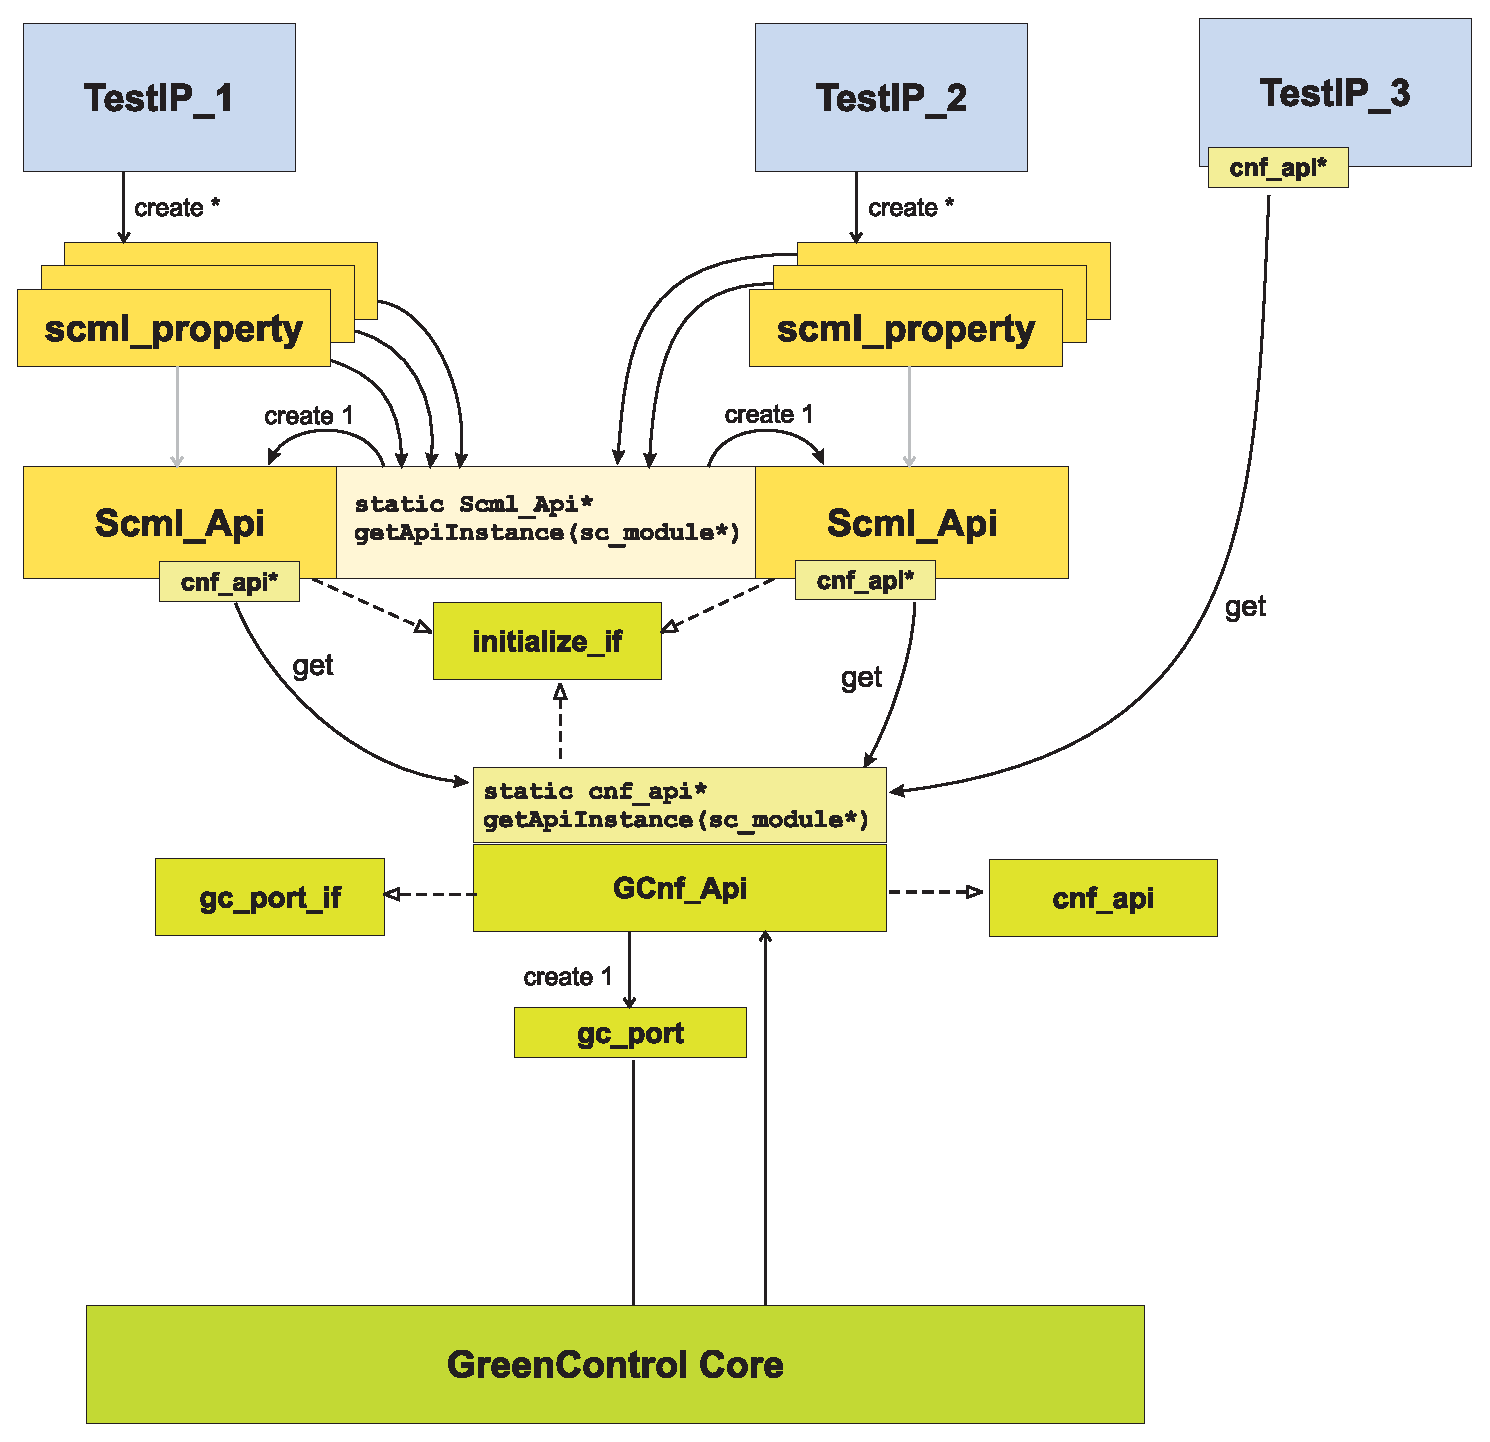
\includegraphics[width=\textwidth]{GreenControlImplMoreApis.eps}}
	\caption{Different concepts according API instances for the SCML API and the GCnf API.}
	\label{fig:GreenControlImplMoreApis}
\end{figure}

See section \ref{StaticGetAPIinstance} for details on the \GreenConfig API's static get instance function.


%%%%%
\subsection{GreenConfig API Interface (cnf\_api\_if)}
\label{GCnfCnfApi}
To achieve independency of the underlying API type (normal \ref{GCnfApi} or private \ref{GCnfPrivateApi}) both APIs implement the class \lstinline|cnf_api_if| which is mainly an interface with virtual functions to be implemented by the APIs and some additional functions implemented in this class. A pointer of type \lstinline|cnf_api_if*| is returned by the \lstinline|getApiInstance| function so the user acts on this one.

Most API functions are virtual and are implemented by the two APIs. Some special functions are independent of the API type and are templated so they cannot be virtual.

Please consider the first two functions are convenience functions but not necessarily the recommended way getting a parameter value, because they are of bad performance:

\begin{itemize}
    \item \lstinline|template<class T> const bool getValue(const std::string &parname, T &value)| \\
    	returns a parameter's value independent of the implicit or explicit status. The string value is converted to the user-chosen template type by using the \lstinline|gs_param| template specialization. This function does only work for types of \lstinline|gs_param<T>|, not for any kind of \lstinline|gs_param_base|, e.g. parameter arrays. \\
	This function calls the virtual \lstinline|std::string getValue(...)| function to get the value from the underlying API. Please consider this function is of bad performance!

    \item  \lstinline|template<class T> const T getValue(const std::string &parname)| \\
    	is a similar function which copies the value instead of writing it to the value parameter. Please consider this function is of bad performance!

    \item \lstinline|template<class T> gs_param<T>* get_gs_param(const std::string &parname)| \\
    	is a convenience function which casts the parameter base object to the user-specified type of \lstinline|gs_param|.

\end{itemize}

%%%%%
\subsection{GreenConfig API (GCnf\_Api)}
\label{GCnf API}\label{GCnfApi}
The \GreenConfig API (class \lstinline|GCnf_Api|) is the native \GreenControl configuration API which provides the functionality of the framework to parameter objects, other APIs or the user directly. The \GreenConfig parameters (\lstinline|gs_param|, see section \ref{GCnfGsParam}) and all other provided configuration APIs make use of this API.

In the example \textsf{user\_api\_example} a simple API is implemented which does {\em not} use this API but uses the \lstinline|gc_port|s directly.

The user should use the  static get function instead (see \ref{StaticGetAPIinstance}) to get an API instance. The default \lstinline|GCnf_Api| object is instantiated by the Config Plugin and should not be instantiated by the user directly.

For a full list of all functions provided by the \GreenConfig API refer to the (doxygen) API reference (see the classes \lstinline|gs::cnf::GCnf_Api_t<...>| and \lstinline|gs::cnf::cnf_api_if|).

%%
\subsubsection{Static get API instance function}
\label{StaticGetAPIinstance}
The \GreenConfig API provides a \lstinline|getApiInstance| method (cf. section \ref{GCnfConceptConfigurationApi}) which returns a pointer to an API instance. This function should be called by a user to get the API instance which is responsible for the module:

\begin{lstlisting}
gs::cnf::cnf_api_if* gs::cnf::GCnf_Api::getApiInstance(sc_module*);
\end{lstlisting}

The returned type \lstinline|gs::cnf::cnf_api_if| is an interface being implemented by the standard configuration API and also by a special API providing private parameters (see section \ref{GCnfPrivateApi}). The user module automatically gets the correct (standard or private) API, accordingly all actions performed on the API pointer automatically respect whether the actions are on private parameters or not.

Only the top-level testbench (or other special tool class) is allowed to call with the parameter being set to NULL -- which will return the default API instance

%%
\subsubsection{Set initial values}
The function \lstinline|bool setInitValue(parname, string value)| sets an initial value (see section \ref{ParamInitValue}) to -- possibly not yet existing, hence implicit -- parameters.

%%
\subsubsection{Lock initial values}
The function \lstinline|bool lockInitValue(parname)| locks an initial value (see section \ref{ParamInitValueLock}) so that this parameter's init value cannot be overwritten by
    any subsequent setInitValue call. This allows to emulate a hierarchical
    precendence since a top-level module can prevent the childs from setting
    init values by locking the init value before creating the subsystem.
   
    Returns false (and does not lock) if parameter is already existing explicitely or if no initial value is existing that can be locked.

%%
\subsubsection{Status is\_used}
With the API function \lstinline|bool is_used(const std::string &parname)| you can check if a parameter has ever been used. It returns \lstinline|true| if the parameter has ever been explicit or the implicit (initial) value has ever been read. This allows for analysis (functional coverage) tools to check after the simulation for e.g. typos in the config file. There is an option for such tools to bypass the status update when calling the API function \lstinline|getValue| by setting \lstinline|not_impact_is_used_status| to \lstinline|true|.


%%
\subsubsection{Parameter access}
Access to any parameter in the system can be done over the API -- as long as the parameter is not private. The standard way accessing a parameter is calling \lstinline|getPar(param_name)| on the API, e.g.

\begin{lstlisting}
gs_param_base* par = mApi->getPar("any_module.param1");
// do some inefficient stuff, see gs_param section
// check if par != NULL
par->setString("10");
std::string val = par->getString();
int ival;
par->getValue(ival);
\end{lstlisting}

If you know the type of the parameter, use e.g.
\begin{lstlisting}
gs_param<int> *par = mApi->get_gs_param<int>("any_module.param1");
// do more efficient stuff, see gs_param section
// check if par != NULL
(*par) = 10;
\end{lstlisting}

The functions \lstinline|getType()| or \lstinline|getTypeString()| can be used to get the type, see section \ref{GCnfGsParam}.

The function \lstinline|existsParam| checks if a parameter is existing explicit or implicit. To check for an explicit parameter, use e.g. \lstinline|if (api->getPar(name) != NULL)|.

Each time \lstinline|api->getPar(name)| is used, it should be checked to be not NULL. If models configure each other it should not be relied on the existence of each other to make the models portable.

There are several functions to get multiple parameters as a vector:\vspace{-2ex}
\begin{itemize}
  \item \lstinline|getParamList(<optional string argument>)| returns a vector of parameter names (strings). Depending on its argument it returns all or a choice of parameters, see the Doxygen documentation for details.
  \item \lstinline|getParams(<optional string argument>)| returns a vector of parameter (base) pointers.
\end{itemize}

%%
\subsubsection{New parameter callbacks}

The macro \lstinline|REGISTER_NEW_PARAM_CALLBACK| can be used to get called for new added parameters.

\begin{lstlisting}
class MyIP_Class
: public sc_core::sc_module {
public:
  // some code [...]
  // Example code to register callback function
  void main_action() {
    // some code, parameters etc...
    my_GCnf_Api.REGISTER_NEW_PARAM_CALLBACK(MyIP_Class, config_callback);
  }
  // Callback function for new added params.
  void config_callback(const std::string parname, const std::string value);
  }
};
\end{lstlisting}

%%
\subsubsection{Parameter callbacks and event notifies}

This API provides the function \lstinline|unregisterAllCallbacks(void* observer)| which uses the \GreenControl command CMD\_UNREGISTER\_PARAM\_CALLBACK. This unregisters the specified observer module from any existing parameter stored in the database. This function is not used by the framework during destruction of an observer but may be used by an user if needed.

\WarningSymbol{Deprecated:} Instead of registering callbacks or getting events for parameter changes at the \GreenConfig API please use directly the parameters to register there, see section \ref{CallbacksAndNotifies}.

%%
\subsubsection{Config API initialize-mode}
\label{ConfigAPIinitializeMode}
The \GreenConfig API may be used during initialize-mode as well as during runtime-mode (see \hyperlink{GCUsersGuide}{\GreenControl User's Guide}).

%In the \GreenConfig API the initialize-mode including the time before initialize-mode is identified by the static member variable
%\begin{lstlisting}
%  static bool initialize_mode;
%\end{lstlisting}

%\vspace{.5 cm}
%\noindent
%\begin{tabularx}{\textwidth}{|l|X|X|}
%	\cline{1-1}\cline{2-2}\cline{3-3}  \lstinline|initialize_mode|        &  true             &  false                          \\
%	\cline{1-1}\cline{2-2}\cline{3-3}                             &  {\em before} initialize-mode\newline and initialize-mode &  runtime-mode\newline during simulation \\
%\hline
%\end{tabularx}
%\vspace{.5 cm}


%%%%%
\subsection{How to make use of the GCnf Api in an API adapter}
This section is about how to develop a new API for some special use by internally using the existing standard GCnf API.
For an example see the Tool GCnf API in directory \Verzeichnis{greencontrol/gcnf/apis/toolApi/}.

\begin{itemize}
  \item The newly developed API file should be placed in an own subdirectory. \GreenConfig APIs are places inside the configuration API directory, e.g. \Verzeichnis{greencontrol/gcnf/apis/my\_api}

  \item The new API has to include the GCnf Api:
\begin{lstlisting}
  #include "greencontrol/config.h"
\end{lstlisting}

	\item The new API has to inherit \lstinline|sc_object| and \lstinline|initialize_if|.

	\item The new API should {\em not} be an \lstinline|sc_module|.

	\item The new API should get a pointer to the \lstinline|GCnf_Api| by calling \lstinline|getApiInstance| only once during instantiation and should store the pointer.
\begin{lstlisting}
  My_Api()
    : sc_object(sc_gen_unique_name("__my_api__"))
  {
    m_gcnf_api = gs::cnf::GCnf_Api::getApiInstance(
                       gs::cnf::get_parent_sc_module(this));
  }
  private:

  /// GCnf_Api which is used by this API
  gs::cnf::cnf_api_if* m_gcnf_api;
\end{lstlisting}

\end{itemize}


%%%%%
\subsection{How to develop an API adapter directly using the gc\_port}
For an example see the Tool API within the \GreenControl example \\
\Verzeichnis{greencontrol/examples/user\_api\_example}.

\begin{itemize}
	\item The newly developed API file should be placed in an own subdirectory. \GreenConfig APIs are places inside the configuration API directory, e.g. \Verzeichnis{greencontrol/gcnf/api/my\_api}
	\item The API can be placed into the namespace {\sffamily gs::cnf}.
	\item The API has to include the configuration include file (for class \lstinline|gs_param_base|):
\begin{lstlisting}
  #include "greencontrol/config.h"
\end{lstlisting}

    \item This examples presumes having used the control and config namespaces:
\begin{lstlisting}
  using namespace gs::ctr;
  using namespace gs::cnf;
\end{lstlisting}

	\item The API has to inherit \lstinline|sc_object|, \lstinline|gs::cnf::initialize_if| and \mbox{\lstinline|gs::ctr::gc_port_if|.}
\begin{lstlisting}
  class My_Api
  : public sc_object, // Better try without!
    public initialize_if,
    public gc_port_if
\end{lstlisting}

	\item The API should {\em not} be an \lstinline|sc_module|.

	\item The interface \lstinline|gc_port_if| has to be implemented (method \lstinline|transport|).

	\item The API has to instantiate the \lstinline|gc_port| to communicate: \mbox{\lstinline|gc_port m_gc_port;|.} The service, which has to be specified in its constructor, has to be set to {\sffamily CONFIG\_SERVICE} (for configuration APIs). The unique API name has to be set and the bool value (if this is a plugin) has to be set to {\sffamily false}. {\sffamily this} has to be given to the port.
\begin{lstlisting}
  My_Api()
    : sc_object(sc_gen_unique_name("__tool_api__")),
      m_gc_port(CONFIG_SERVICE, MY_API_NAME, false, this)
  {
  }
\end{lstlisting}

	\item The interface \lstinline|initialize_if| \emph{can} be be implemented and can be used to identify the initialize-mode and to do initial configuration if this is not possible at construction.

\end{itemize}


%%%%%
\subsection{GreenConfig private API (GCnf\_private\_Api)}
\label{GCnfPrivateApi}

The \GreenConfig private API (class \lstinline|GCnf_private_Api|) is a special API that allows private parameters. The private API implements the interface \lstinline|gs::cnf::cnf_api_if| and can be used exactly as the normal API.

A module which should hide its parameters and the ones of its childs can instantiate a private API. This API is registered at the static \lstinline|getApiInstance| function. If one of the parameters or child modules call the static \lstinline|getApiInstance| function it will return the private API. The private API has an internal parameter database similar to the configuration service plugin.

The user can give parameters to the private API that should {\em not} be private by giving their local names to the private API constructor.

Hierarchies of private APIs are possible, see figure \ref{fig:GCnfDatabaseHierarchyConcept}. More details are shown in figure \ref{fig:GCnfDatabaseHierarchy}.

\begin{figure}[htbp]
	\centerline{
		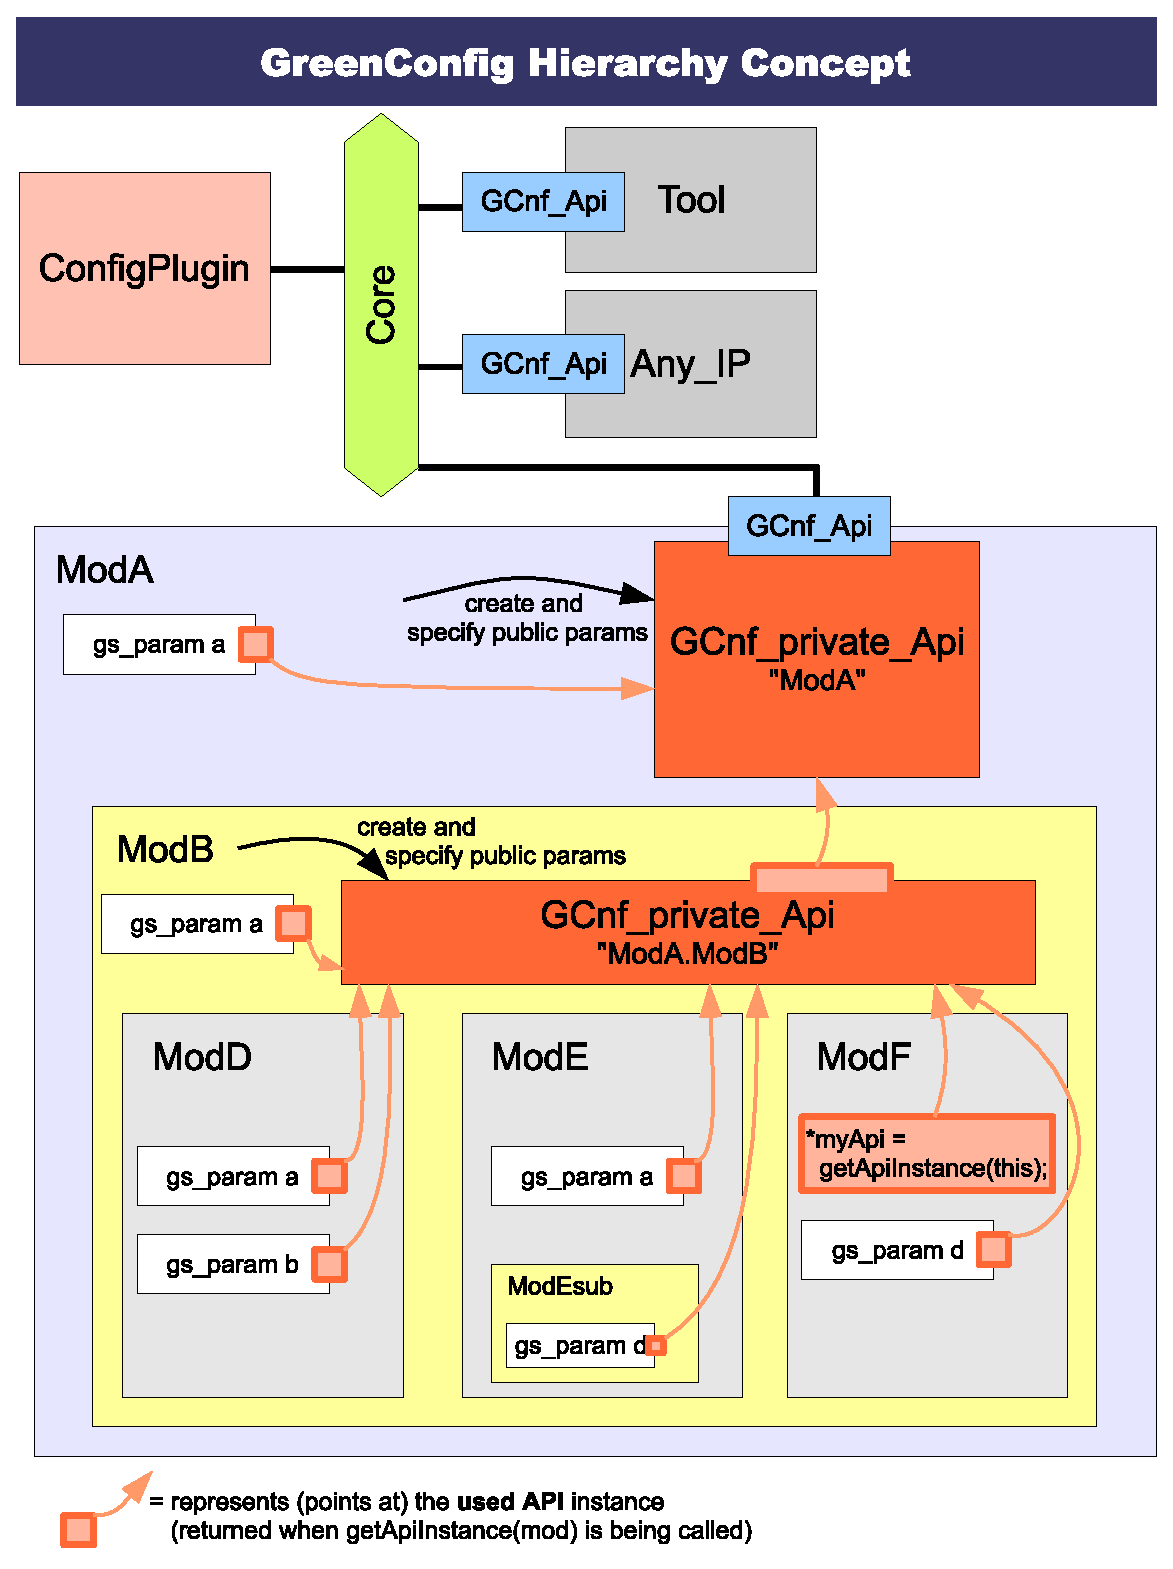
\includegraphics[width=14cm]{DatabaseHierarchyConcept.eps}}
	\caption{Concept database hierarchy with private APIs.}
	\label{fig:GCnfDatabaseHierarchyConcept}
\end{figure}

\begin{landscape}
\begin{figure}[htbp]
	\centerline{
		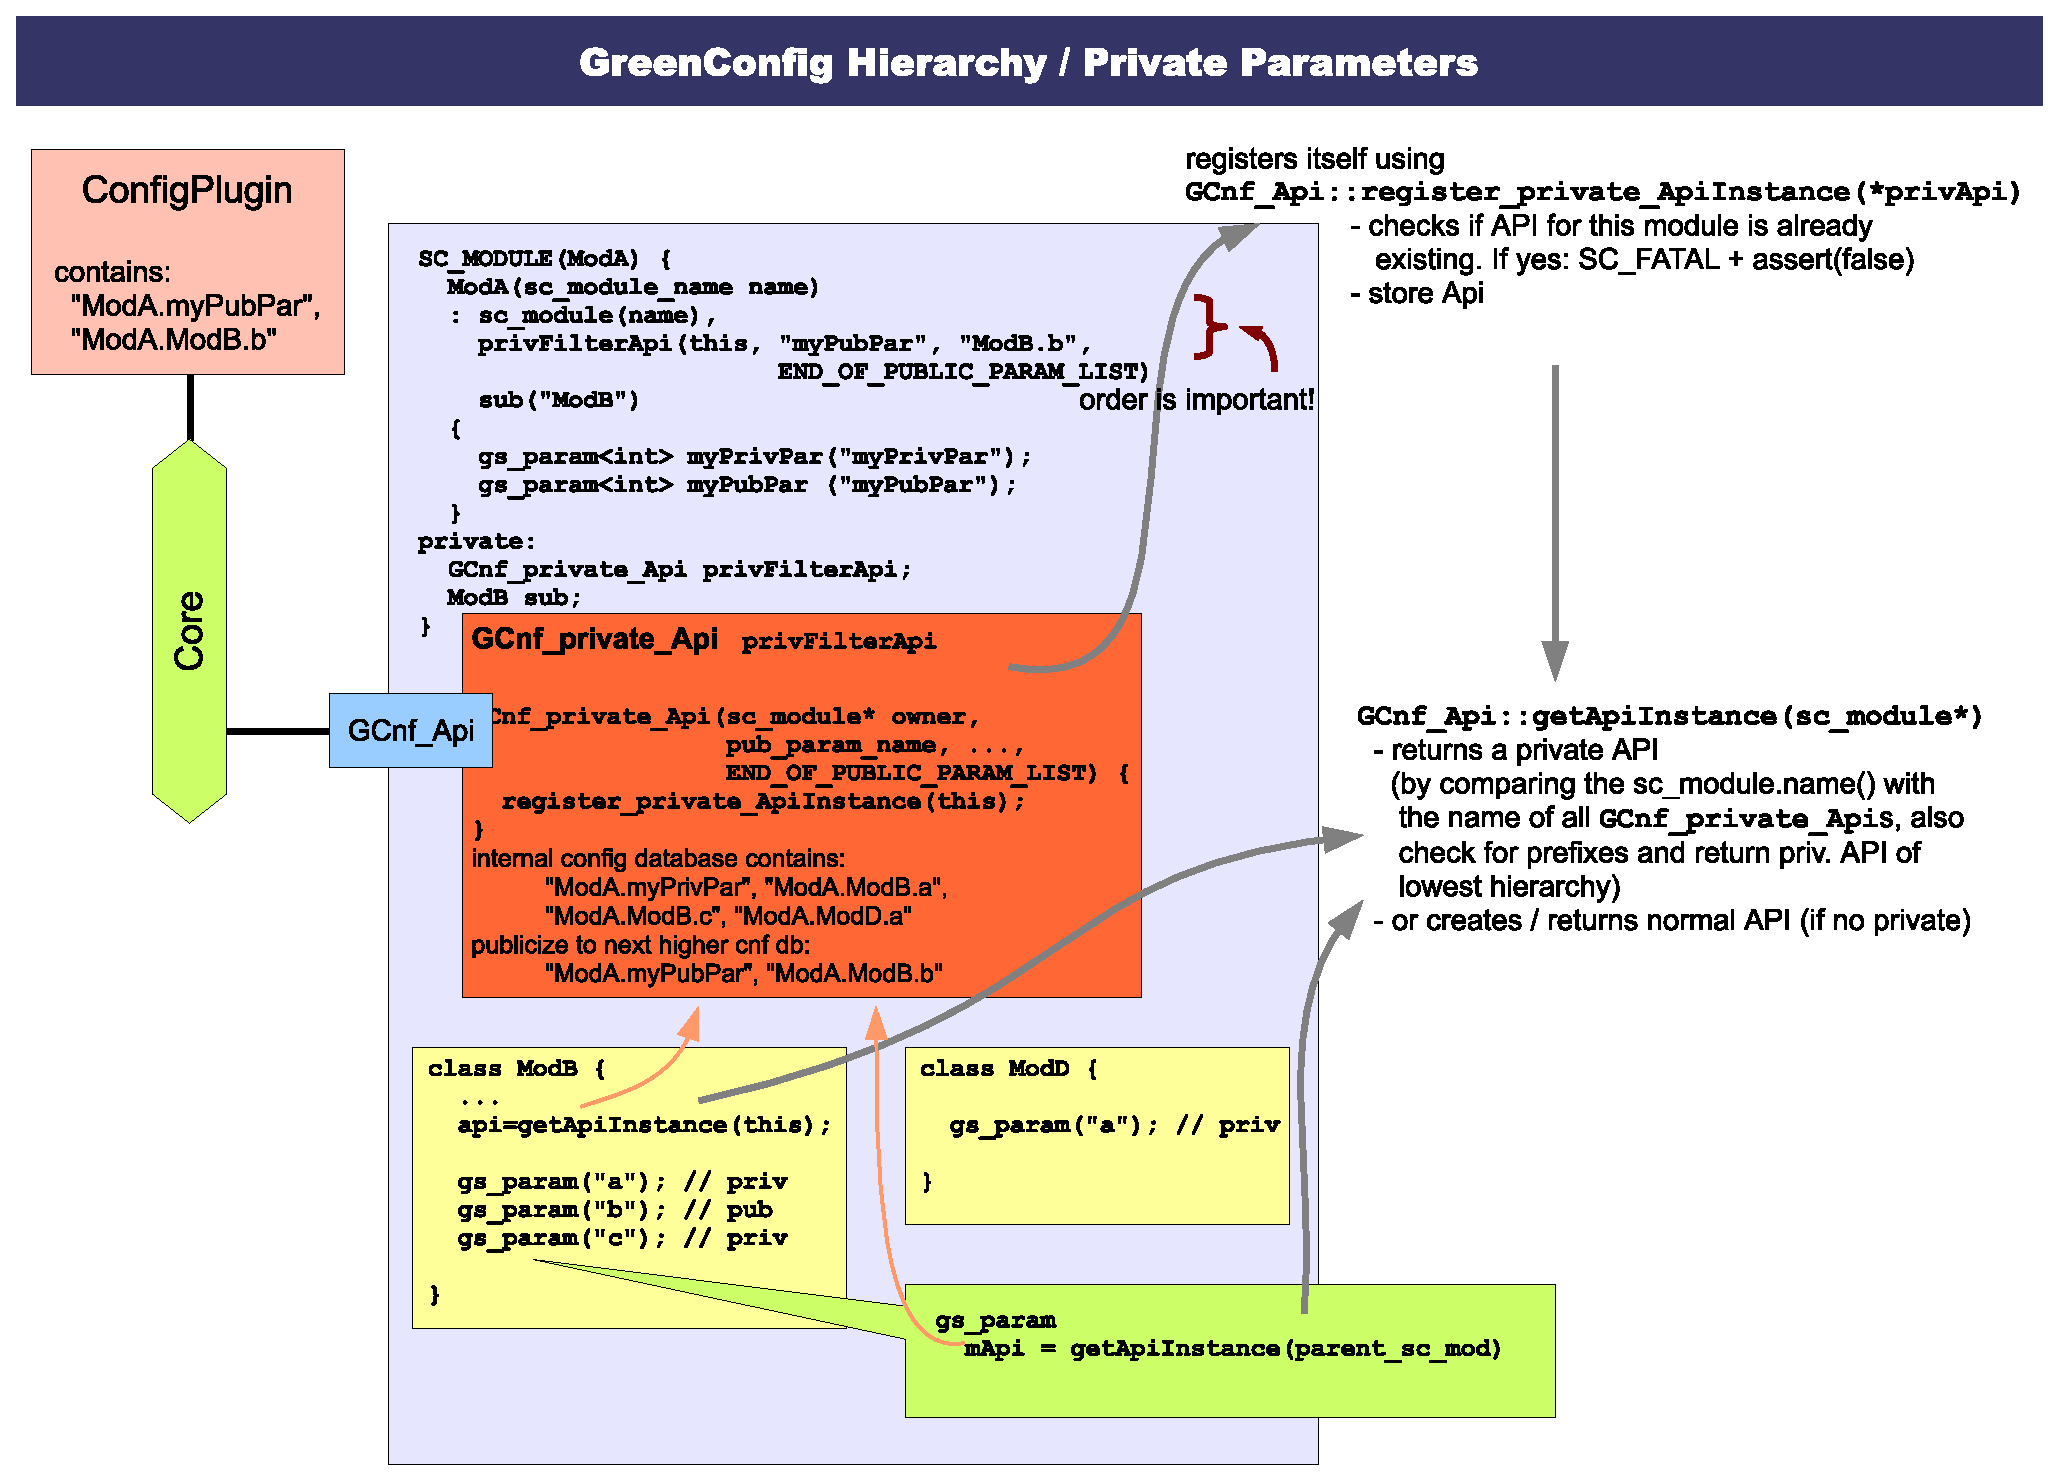
\includegraphics[width=20cm]{DatabaseHierarchy.eps}}
	\caption{Database hierarchy with private APIs.}
	\label{fig:GCnfDatabaseHierarchy}
\end{figure}
\end{landscape}

\paragraph{Usage}
The example below shows a module ({\sffamily ModA}) which creates a private API ({\sffamily privFilterApi}). That API makes all parameters  of {\sffamily ModA} and parameters of its submodules private. Additionally calling \lstinline|getApiInstance(mod)| returns this private API as long as {\sffamily mod} is a pointer to the owning module or one of its child modules. Exclusions are the two parameters {\sffamily myPubPar} and {\sffamily ModB.b}.

The {\em instantiation order} is important: First instantiate the private API, afterward instantiate any parameters and submodules.

The private API object must exist at least as long as any parameter or child module which is accessing this API exists.

When constructing the private with specifying public parameters, the constructor with variable arguments is the default one. Use \lstinline|END_OF_PUBLIC_PARAM_LIST| to finalize the parameter name list. The parameter names are {\em local parameter names}! The default constructor is:
\begin{lstlisting}
GCnf_private_Api(sc_module* owner_module, const char* pub_par ...);
\end{lstlisting}

Alternatively the constructor without public parameters can be used:
\begin{lstlisting}
GCnf_private_Api(sc_module* owner_module);
\end{lstlisting}

At the end the constructor getting the parameter name list as a vector can be used instead of the on with variable arguments:
\begin{lstlisting}
GCnf_private_Api(sc_module* owner_module,
                 std::vector<std::string> pub_params);
\end{lstlisting}

The module pointer must point to a valid module. Private top level parameters are not supported.


\begin{lstlisting}
class ModA
  : public sc_module {
  [...]
  ModA(sc_module_name name)
  : sc_module(name),
    privFilterApi(this, "myPubPar", "ModB.b", END_OF_PUBLIC_PARAM_LIST),
    sub("ModB"),
    int_param("int_param", 45),
  {
    gs_param<int> myPrivPar("myPrivPar");
    gs_param<int> myPubPar ("myPubPar");
  }
private:
  gs::cnf::GCnf_private_Api privFilterApi;
  ModB sub;
  gs::gs_param<int>   int_param;
}
\end{lstlisting}

\noindent
\begin{minipage}{\textwidth}
Submodules need not to be aware of the private API and can instantiate parameters and get their API pointer normally. The private API will be used automatically.

\begin{lstlisting}
class ModB
  : public sc_module
  {
  public:
    SC_HAS_PROCESS(ModB);
    ModB(sc_module_name name)
    : sc_module(name),
      submod("AnotherSubModule"),
      b("b", 1111),
    {
      mApi = gs::cnf::GCnf_Api::getApiInstance(this);
    }
  protected:
    AnotherModule submod;
    gs::gs_param<int> b;
    gs::cnf::cnf_api_if *mApi;
  };
\end{lstlisting}
\end{minipage}

%%
\subsubsection{Implementation}
A private API calls the static \lstinline|getApiInstance| function during construction before registering itself. Accordingly the private API gets a pointer to the next API upwards responsible for the owning module ({\em parent API}). This may be the (one) normal top-level API but this also may be another private API. This allows to build a hierarchy of private APIs.

API calls according the specified public parameters are forwarded to the parent API, all other calls are directed to an internal private config database which is like the config service plugin. The communication does not use transactions but function calls to make it less vulnerable. The private API checks for each call whether to forward it to the parent API or whether to process it locally. There are also some calls that are mixed (e.g. \lstinline|getList()| returns a combination of the parent and the private list).

%TODO: To be extended

%%%%%
\subsection{GreenConfig parameters: gs\_param}
\label{GCnfGsParam}

The main interface a normal user gets in touch with when using the \GreenConfig framework are the \GreenConfig parameters, called {\em gs\_param}.

\paragraph{Usage}The favored parameters that should be used when a new configurable IP is developed are the \GreenConfig parameters in the class \lstinline|gs_param|.

The \lstinline|gs_param| class is -- additional to the configuration namespace {\sffamily gs::cnf} -- also available within the GreenSocs namespace {\sffamily gs}.

These parameters support the whole functionality of the \GreenConfig API (\lstinline|GCnf_Api|) and
can  be used just like the data types they represent.

New data types can be added by creating template specializations (\lstinline|gs_param<T>|).  \newline  The supported data types are:

\begin{itemize}
	\item {\sffamily int}, {\sffamily unsigned int}, {\sffamily bool}, {\sffamily double}, {\sffamily float},
		{\sffamily string}, {\sffamily unsigned long long}, {\sffamily long long}, {\sffamily unsigned char}, {\sffamily unsigned short}, {\sffamily char}, {\sffamily signed char},
		{\sffamily sc\_int\_base}, {\sffamily sc\_int}, {\sffamily sc\_uint\_base}, {\sffamily sc\_uint},
		{\sffamily sc\_signed}, {\sffamily sc\_bigint}, {\sffamily sc\_unsigned}, {\sffamily sc\_biguint},
		{\sffamily sc\_logic} \newline
		(with specialized classes including all operators)
	\item {\sffamily sc\_attribute\textless T\textgreater} with T= all other supported types
    \item {\sffamily sc\_bit} are deprecated, use bool instead.
    \item {\sffamily sc\_time} can deserialize the following strings to sc\_time:
	\begin{itemize}
		\item ``$<$double value$>$'' $\rightarrow$ Convert to seconds \newline
		(reverse way of the \lstinline|sc_time::to_double()| function) \newline
          Example: \lstinline|my_param.setString("0.000000025"); // sets value to 25 ns |
		\item ``$<$uint64$> <$sc\_time\_unit$>$'' (reverse way of \lstinline|sc_time::to_string()| function) \newline
          Example: \lstinline|my_param.setString("25 ns"); // sets value to 25 ns| \newline
          Example: \lstinline|my_param.setString("25 SC_NS"); // sets value to 25 ns|
	\end{itemize}
	\item {\sffamily std::vector$<$std::string$>$} serializes a vector to e.g.
		\begin{lstlisting}[language=TeX]
{"This","is the","simplest","example"}
{"example","with","quotes \"here\" inside and comma, here","and single quote 'here"}
		\end{lstlisting}
		Syntax to set the string representation of such a parameter:

		Example C++ code:
		\begin{quote}
		\lstinline|vecLocal.setString(std::string("{\"example\", \"with\", \"quotes \\\"here\\\" inside and comma, here\", \"and single quote 'here\" }"));|
		\end{quote}
		Example config file (not-lua):
		\begin{quote}
		\begin{lstlisting}[language=TeX]
IPVec.vec5 "{ "with", "quotes in \\"this\\"." }"
## we need this double \\ syntax to be the same as in code (\" needs to be in the resulting string being set)
		\end{lstlisting}
		\end{quote}
	\item All data types which support the stream operators may be used as template specialization for \lstinline|gs_param|.
\end{itemize}

Before the parameters can be used the developer has to include the parameter class (see file \Datei{greencontrol/gcnf/apis/gs\_param/gs\_param\_class.h}) by including \Datei{greencontrol/config.h}.

Parameters are derived from a base class \lstinline|gs_param_base| which can be used each time the type does not matter or is not known, e.g. as a function's parameter or return value.
The \lstinline|gs_param_base| class is -- additional to the configuration namespace {\sffamily gs::cnf} -- also available within the GreenSocs namespace {\sffamily gs}.


Usage:

\begin{lstlisting}
  gs::gs_param<int> int_param("my_par_name", "104");
// or
  gs::gs_param<int> int_param("my_par_name", 104);
\end{lstlisting}

Usage as member variables:

\begin{lstlisting}
class MyIP
: public sc_module
{
public:

  SC_HAS_PROCESS(MyIP);
  MyIP(sc_module_name name)
    : sc_module(name),
      int_param ("int_param"),
      uint_param ("uint_param", 1000) // with default
  {   }

  /// Example parameters.
  gs::gs_param<int>           int_param;
  gs::gs_param<unsigned int>  uint_param;
};
\end{lstlisting}

Some different {\em constructors} may be used to instantiate a \lstinline|gs_param|:

\begin{itemize}
	\item Constructor with the name of the parameter,
	\item Constructor with the name and the {\em default value} (value type or string representation).
\end{itemize}

The constructor without name is private and cannot be used because it results in an unnamed parameter.

For integer values hexadecimal notation may be used.

The {\em operators} \colorbox{hellgrau}{$=$}, \colorbox{hellgrau}{$+$}, \colorbox{hellgrau}{$-$}, \colorbox{hellgrau}{$/$}, \colorbox{hellgrau}{$*$}, \colorbox{hellgrau}{$+=$}, \colorbox{hellgrau}{$-=$}, \colorbox{hellgrau}{$/=$}, \colorbox{hellgrau}{$*=$}, \colorbox{hellgrau}{$\%=$}, \colorbox{hellgrau}{$\hat{ }=$}, \colorbox{hellgrau}{$\&=$}, \colorbox{hellgrau}{$|=$}, \colorbox{hellgrau}{$<<=$}, \colorbox{hellgrau}{$>>=$}, \colorbox{hellgrau}{$--$} (prefix, postfix), \colorbox{hellgrau}{$++$} (prefix, postfix) are (as possible) available for the supported data types, see itemization above.

Also the conversion operator \lstinline|gs_param<T>::operator const T& ()| is implemented.

For purposes of \GreenAV (Analysis and Visibility service plugin) there are the operators \colorbox{hellgrau}{$+$}, \colorbox{hellgrau}{$-$}, \colorbox{hellgrau}{$/$}, \colorbox{hellgrau}{$*$} for the parameter base class \lstinline|gs_param_base|. The operators (called 'convenient operators') return a tripple which is used by the Calculator in \GreenAV.

In most cases the parameter instance may be used like the data type it represents. To get the value, simply use the parameter variable, and to set the value use the = operator. If that does not work (e.g. for not explicit supported data types) use the data type methods \lstinline|setValue(T)| and \lstinline|const T& getValue()|.

Operators \colorbox{hellgrau}{$==$} may be used to compare parameters of same type to each other or with objects of their type. Examples:
\begin{lstlisting}
gs::gs_param<bool> myBoolParam1, myBoolParam1; // initialization skipped
bool result = (myBoolParam1 == myBoolParam2);
bool result2 = (myBoolParam1 == result);
bool result3 = (result2 == myBoolParam2);
\end{lstlisting}


% removed due to security reasons! All API functions can be accessed through the call \lstinline|my_gs_param.getApi()|.

%%
\ZwischenUberschrift{Parameter string representation}
To {\em get} and {\em set} with string representation of the values the methods \lstinline|setString(const string&)| and \lstinline|const string getString()| can be used. See the doxygen documentation for rules for each parameter type.

The parameter string set functions support the environment variable substitution which is described in section \ref{ConfigFileTool} (cf. section \ref{sec:ParamImplementation}).


%%
\ZwischenUberschrift{Parameter attributes}
Parameters may have a set of attributes which give more information about their usage within the model.

Parameter attributes (\lstinline|gs::cnf::param_attribute|) (don't mistake them for {\sffamily sc\_attributes}) are simple \lstinline|unsigned int|s, represented with an enumeration: \lstinline|gs::cnf::param_attributes::param_attribute_enum|. The possible types are: (TODO) {\sffamily config, runtime\_config, elab\_config, read\_only, analysis, temp, output, internal}.

Parameters provide the following functions to give access to the attributes:
\begin{itemize}
	\item \lstinline|bool add_param_attribute(const param_attribute attr)|  \newline
	adds a parameter attribute.

	\item \lstinline|bool has_param_attribute(const param_attribute attr) const| \newline
	 returns if a special parameter attribute is set.

	\item \lstinline|const std::set<param_attribute> get_param_attributes() const|  \newline
	returns a set containing all parameter attributes that are set for this param.

	\item \lstinline|bool remove_param_attribute(param_attribute attr)|  \newline
	removes a parameter attribute.

	\item \lstinline|void remove_all_param_attributes()|  \newline
	removes all parameter attributes of this parameter.
\end{itemize}

The following listing shows how to use the parameter attributes:
\begin{lstlisting}
  gs::gs_param<int> p("param");
  p.add_param_attribute(gs::cnf::param_attributes::config);      // add
  p.add_param_attribute(gs::cnf::param_attributes::output);      // add
  if (p.has_param_attribute(gs::cnf::param_attributes::config))  // check
    /* do something */
  set<gs::cnf::param_attribute> s = p.get_param_attributes();  // get all
  p.remove_param_attribute(gs::cnf::param_attributes::output); // remove
  p.remove_all_param_attributes(); // remove all
\end{lstlisting}

%%
\ZwischenUberschrift{Parameters not registered at the database}
There may be situations where it is reasonable to create parameters that are not registered at the database (regardless whether this is the normal or a private one). The advantages of parameters can be used without the need of making them accessible via the API and plugin (database).

\WarningSymbol{} Be careful when using these parameters, normally standard parameters should be used!

Two special constructors are available to create such parameters (simplified view). The name and value need to be provided as strings.
\begin{lstlisting}
gs_param(string &name, string &value, gs_param_array* parent_array,     bool force_top_level_name, bool register_at_db);
gs_param(string &name, string &value, gs_param_array& parent_array,     bool force_top_level_name, bool register_at_db);
\end{lstlisting}


%%
\ZwischenUberschrift{Parameters as array members}
Another set of constructors can be used to create parameters as extended array members. See section \ref{ExtendedParameterArray} for details.

%%
\ZwischenUberschrift{Parameter base class gs\_param\_base}
Some functions in the configuration framework return the base class of the specialized parameter class if type independency is needed (e.g. callbacks).

A pointer/reference to a parameter base object (\lstinline|gs_param_base|) can be useful in different ways:

\begin{itemize}

  \item Give it directly to many available functions that get parameter bases.

  \item Get the string representation of the parameter's value: \lstinline|string getString()|

  \item Set the the parameter's value using its string representation: \lstinline|bool setString(val_str)|

  \item Get the value already converted to the right type. The awaited type \lstinline|T| must be known: \newline
  	\lstinline|bool getValue<class T>(T &value)| (returning the success of the conversion) or \newline
	\lstinline|T getValue<class T>()| (one more memory allocation because of copying the return value).

  \item Get the parameter pointer already converted to the right type: \newline
  	\lstinline|gs_param<T>* get_gs_param<class T>()|

  \item Convert to the {\em unknown} template type: \newline
  	The base class \lstinline|gs_param_base| has two functions to get the original type of the object which allows the user to cast the base object to the correct parameter object: \lstinline|getType()| returns an enumeration \lstinline|Param_type| which may be used in an switch case statement. This function returns reasonable values for the supported data types. When using user specialized data types the function \lstinline|getTypeString()| may be used. There a string describing the type is returned.

\end{itemize}

For more details about how to use parameters see the \GreenConfig Tutorial.


\paragraph{Parameter Base: get void* value}
The virtual function
\lstinline|virtual void* get_value_pointer()|
can be used to cast the value to a base class of the value, e.g. cast an \lstinline|sc_int<length>| to \lstinline|sc_int_base|.

A use case are SystemC data types where it is not possible to cast a \lstinline|gs_param_base| to the corresponding type, e.g. \lstinline|gs_param<sc_int<10> >|. In this case call \lstinline|get_value_pointer()| on the base parameter and cast the result e.g. to \lstinline|sc_int_base|.

Example:
\begin{lstlisting}
void callback(gs::gs_param_base &par) {
  switch (par.getType) {
    case gs::cnf::PARTYPE_SC_SIGNED:
    case gc::cnf::PARTYPE_SC_BIGINT:
      void* pv = par.get_value_pointer();
      sc_signed* p = static_cast<sc_signed*>(pv);
      // Do something with p->length() and p->to_uint64() etc.
  }
}
\end{lstlisting}


\paragraph{Parameter names} \hypertarget{GCnfParameterNames}
Users creating parameters should use {\em parameter names} matching the SystemC naming rules. A parameter name should not include SystemC name delimiters (e.g. dots for OSCI implementation).

\WarningSymbol{} But delimiters are not forbidden, a user who knows what he is doing is allowed to use delimiters!

There is the possibility to {\em choose the name of a parameter fully free} of the hierarchical position of the owning module. Even within a module it is possible to choose a arbitrary name (matching the naming rules, including delimiters) and prevent the parameter from attaching the name prefix of the owning module. In this case the {\sffamily sc\_object} is still a child of the creating module, only the parameter's name may be in a different hierarchy position. To do this use the constructor parameter \lstinline|force_top_level_name| which is an optional parameter for various constructors, see the (doxygen) API reference.

\WarningSymbol{} This feature may confuse users and should be used carefully!

\paragraph{Top-level parameters}
Parameters are allowed to be instantiated at top-level (outside the SystemC hierarchy), e.g. in {\sffamily sc\_main}. Here the same \hyperlink{GCnfParameterNames}{parameter naming rules} are applied as for not top-level parameters.

\WarningSymbol{} Be careful not to cause name collisions with existing SystemC modules and their parameters when using hierarchical parameter names with delimiters in them.

\paragraph{Parameter name collisions} Since each parameter name is unique in the database, it is an error to create more than one parameter with complete identical names. This could happen when setting top-level parameter names manually. During creation of the doubled parameters there will be an sc\_warning. Initial values are applied to all parameters (matching the given name) that are tried to add to the database now, even if they are already existing and adding fails. It is strongly recommended not to use such not added parameters but resolve the naming collision.


%%
\subsubsection{Callbacks}
\label{CallbacksAndNotifies}

This section is about how the user and APIs can be notified about parameter changes and other actions on parameters using function callbacks (sc\_event-based notifies are deprecated).

Each parameter handles an own list of callbacks and an event notification.
These notifies can be received by any object. E.g. a tool can be notified on all changes of any parameter.

\paragraph{Event} (deprecated) The parameter object is able to return a reference to an {\em sc\_event} which is notified each time the parameter value changes: \lstinline|sc_event& getUpdateEvent()|.

\paragraph{Callback} A callback function can be registered and unregistered with the parameter. This is the preferred way due to performance reasons. Callbacks also work before simulation runtime. 


\paragraph{Callback types} There are different callback types (enum \lstinline|callback_type|):

\noindent
\begin{tabularx}{\textwidth}{|p{3.6cm}|X|}
	\hline
    \lstinline|pre_read| & Calls before a parameter value is been read. Value can be updated here. \\
	\hline
    \lstinline|post_read| & Calls while a parameter is read. Value shall not be updated within this callback\footnote{Technically this is not really a post\_read because the get function not yet returned to the user. Even the actual read from the containing value within the parameter might not have been done yet if it is done directly within the return statement.} \\
	\hline
    \lstinline|reject_write| & Calls before the parameter value will be written to -- allows the callee to reject the write. \\
	\hline
    \lstinline|pre_write| & Calls before the parameter value will be definitely written to (not being rejected). \\
	\hline
    \lstinline|post_write| & Calls after the parameter value write is done. \\
	\hline
    \lstinline|create_param| & Calls when a new (implicit or explicit) parameter is created (to be registered with the GCnf\_API, not a parmeter).\\
	\hline
    \lstinline|destroy_param| & Calls when the parameter is to be destroyed. \\
	\hline
\end{tabularx}


\WarningSymbol{Note}: There is no post callback following a pre callback if the action failed.

Callbacks can be registered for any method with the signatures
\begin{lstlisting}
gs::cnf::callback_return_type config_callback(gs::gs_param_base& changed_param, gs::cnf::callback_type reason)
\end{lstlisting}
and register it at the parameter as callback function for this parameter. One callback function may be registered at several parameters and several callback functions may be registered at one parameter. %The callbacks work during initialize-mode.

Inside callback functions it is forbidden to use wait statements.

Callback functions can be registered at a parameter with:
\begin{lstlisting}
GC_REGISTER_TYPED_PARAM_CALLBACK(&my_param, callback_type, class_name, callback_method_name)
\end{lstlisting}

To enable a module being able to register callbacks, use the macro \lstinline|GC_HAS_CALLBACKS()| in the module's body. This macro creates a member variable which stores the created callback adapters to be able to unregister them when destructing the module. In addition to this the macro creates a help function which is needed when registering a callback.

The user module needs to call the macro \lstinline|GC_UNREGISTER_CALLBACKS()| in its destructor.
With this macro all callbacks that were registered by this module will be unregistered. A shared pointer is used to hold the adapter instance to ensure that it is destroyed when all interested instances (parameter and observer module) are destroyed or unregistered.

Optional: If the user takes care to unregister all callbacks himself this callback needs not to be used - but it may be used in addition. If there is no reason to leave it out, use it!

\begin{lstlisting}
class MyIP2 {
  GC_HAS_CALLBACKS();
  MyIP2() { ... }
  ~MyIP2() {
    GC_UNREGISTER_CALLBACKS();
  }
  ...
}
\end{lstlisting}

The following sniped is an example where IP1 has parameters which are observed by IP2 and IP3 (see \Verzeichnis{greencontrol/examples/callback\_example}).

\begin{lstlisting}
void MyIP2::main_action() {
  // Register post_write-callback for parameter int_param in module IP1
  GC_REGISTER_TYPED_PARAM_CALLBACK(m_Api->getPar("IP1.int_param"), gs::cnf::post_write, MyIP2, cnf_callback);
  // Register pre_read-callback for parameter str_param in module IP1 with keeping the callback adapter pointer
  boost::shared_ptr<gs::cnf::ParamCallbAdapt_b> cbAdapt;
  cbAdapt = GC_REGISTER_TYPED_PARAM_CALLBACK(m_Api->getPar("IP1.str_param"), gs::cnf::pre_read, MyIP2, cnf_callback);
}

// Callback function with default signature.
gs::cnf::callback_return_type MyIP2::cnf_callback(gs::gs_param_base& changed_param, gs::cnf::callback_type reason) {
  gs::cnf::callback_return_type cb_return = gs::cnf::return_nothing;
  switch (reason) {
    case gs::cnf::pre_read:
      // Here you could update the parameters value to whatever the reading object should see
      break;
    case gs::cnf::reject_write:
      // Here you could reject the write if it does not match some requirements, e.g. parameter dependencies
      if (reject) cb_return = gs::cnf::return_value_change_rejected;
      break;
    case gs::cnf::pre_write:
      // Here you could log the old value
      std::cout << "   callback function: (old value: "<<changed_param.getString()<<")" << std::endl;
      break;
    case gs::cnf::post_write:
      // Here you could log the new value
      std::cout << "   callback function: (new value: "<<changed_param.getString()<<")" << std::endl;
      break;
    case gs::cnf::destroy_param:
      // Here you should remove your local reference/pointer to this parameter to prevent from using it later (seg faults!)
      break;
    default:
      // nothing else possible
      // Note: create_param is called to a different method with different signature
      break;
  }
  return cb_return;
}
\end{lstlisting}

As can be seen in the example the register call returns a boost shared pointer to a parameter callback adapter (\lstinline|boost::shared_ptr<gs::cnf::ParamCallbAdapt_b>|). This adapter pointer {\em may} be kept by the use module if it needs to unregister the callback {\em before} destruction of the module.

The callback function gets a reference to the base class of the parameter. The user can get the value directly only via a string (calling \lstinline|getString()|). The base class can be casted to the specialized \lstinline|gs_param| object using the \lstinline|getType()| or \lstinline|getTypeString()| functions.

The callback function must check the \lstinline|is_destructing()| function on the parameter to check whether this is a callback to inform about the destruction of the parameter!

\paragraph{Callback order} The callback order is the registering order (since \GreenControl release 3.0.0).

\paragraph{Unregister callbacks}   A callback that was registered at a parameter can be unregistered in different ways. The default way is item one. You need not to use the other ones!

\begin{enumerate}
  \item {\em Default}: \newline
  \lstinline|GC_UNREGISTER_CALLBACK(boost::shared_ptr<gs::cnf::ParamCallbAdapt_b> callb)| \newline
Unregister a callback whose callback adapter pointer (shared pointer) is available in the user module.
  \item Use the \GreenConfig API call \lstinline|my_Api.unregisterAllCallbacks(void* observer)| \newline
Unregister all callbacks the observer module (whose this pointer must be specified) has registered at any parameter in the system. This call uses the config plugin to call the unregister function of each existing parameter in the system.
  \item \lstinline|myparam.unregisterParamCallbacks(void* observer)| \newline
Unregister all callbacks the observer module has registered at this (myparam) parameter.
This function is used by the config plugin when performing a the API call of item two and may be called directly by the user, too.
\end{enumerate}

\WarningSymbol{Attention}: The callback function should take care when setting the parameter's value because that could result in a new callback of the same function which means an endless loop.

\WarningSymbol{Attention}: During a callback it is safe to unregister the current callback adapter. But unregistering further callbacks of that parameter can cause a segmentation fault because the parameter's callbacks are just called. If the parameter is destructing  (destroy\_param callback or \lstinline|is_destructing()| returns true) it is fase to remove any callback of that parameter (and of course of any other parameter, too) because here a (slower) safe callback function is used.

\paragraph{Background destruction mechanism for callbacks}
The issue why the destruction mechanism with the macro \lstinline|GC_UNREGISTER_CALLBACKS(mGCnfApi)| is needed for observer modules which register parameter callbacks is: 1. An observer module registers a callback at a parameter. 2. The observer module gets destroyed. 3. The parameter still has the callback registered: on changes or even on destruction of the parameter it tries to call the observer - which is already destructed 4. $\Rightarrow$ segmentation fault

So the observer module must assure that each callback it has registered at any parameter is unregistered when the module gets destroyed!

The way chosen:
\begin{itemize}
  \item Each observer module holds a list of its parameter callback adapters. This list is initialized by the macro \lstinline|GC_HAS_CALLBACKS()| which must be used in the class body of the module that registers callbacks.
  \item When a new callback is registered at any parameter this callback adapter is added to the module's list.
  \item During destruction of the module these adapters are deleted. This is done by the macro \lstinline|GC_UNREGISTER_CALLBACKS()| which must be added to the module's destructor.
  \item During their destruction the adapters inform their parent parameter (they have a pointer to it) to remove themselves from the parameter's callback list.
\end{itemize}

Another possible way:
\begin{itemize}
  \item During callback registering the created parameter callback adapter stores the pointer to the observing module.
  \item When destructing the module, a macro could send the this pointer of the module to the ConfigPlugin via the API.
  \item The ConfigPlugin calls <code>unregisterCallbacks(pointer)</code> on each known parameter.
  \item Each parameter searches for callback adapters which have the observer pointer set to that pointer and delete that adapters and callbacks.
\end{itemize}

%%
\subsubsection{Implementation}\label{sec:ParamImplementation}
This section is about the implementation of the \GreenConfig parameters and how to add template specializations.

The base class {\bf \lstinline|gs_param_base|} is not templated. It has member variables for the
parameter name and the parent name which is used in the constructor (when no name is set) and for debug. The \GreenConfig API variable is also a member of this base class. It is generated with the pointer of the next child object which is an sc\_module. The member variables are protected to allow access by derived classes. The constructor instantiates the API instance using the static function \lstinline|GCnf_Api::getApiInstance(mod)| (see section \ref{StaticGetAPIinstance}) and sets the parameter (and parent) name. The value-independent observer function is in this base class, too.

The template class {\bf \lstinline|gs_param_t|} inherits \lstinline|gs_param_base| and extends it for some functionality which is dependent on the value type (operators, set and get value methods). All methods which need a conversion between value type and string representation make use of the virtual methods \lstinline|serialize| and \lstinline|getValue|.

The template class {\bf \lstinline|gs_param|} inherits \lstinline|gs_param_t|. The template specializations should implement the operators (for the specialized data type) and must implement the conversion methods \lstinline|serialize| and \lstinline|getValue| to achieve a specialized conversion for the data type.

If no explicit specialization for the desired data type exists, there is the default \lstinline|gs_param<T>| implementation. There the operators except the = operator are not available. Conversion is done per default with string streams.

\ZwischenUberschrift{How to make a new parameter type}
If a specialization for a user data type (or an existing but not yet supported data type) is needed, the class
\mbox{\lstinline|gs_param<T>|} can be specialized for the needed data type T. The functions needed
to be specialized are: 
\begin{itemize}
  \item type information functions, 
  \item \lstinline|serialize|, 
  \item \mbox{\lstinline|static_deserialize|.} 
\end{itemize}
The macro \lstinline|GS_PARAM_HEAD| creates some using statements, many constructors, the destructor and the non-static deserialize function which calls the user-implemented static one (for details see \Datei{greencontrol/gcnf/apis/gs\_param/gs\_param.h}). You also may (but need not) use operator macros. 

It is recommended to use a class body similar to the existing specializations:
\begin{lstlisting}
template<>
class gs_param<my_data_type>
: public gs_param_t<my_data_type>
{
  /// Typedef for the value.
  typedef my_data_type val_type;

public:
  GS_PARAM_HEAD;

  //  operators
  GC_SPECIALISATIONS_ARITHMETIC_OPERATORS;
  GC_SPECIALISATIONS_BINARY_OPERATORS;
  GC_SPECIALISATIONS_INCREMENT_OPERATORS;
  GC_SPECIALISATIONS_DECREMENT_OPERATORS;

  /// Overloads gs_param_base::getTypeString
  const std::string getTypeString() {
    return string("my_data_type");
  }
  /// Overloads gs_param_base::getType needs not to be overloaded
  //  because enum does not contain my type anyway
  //const std::string getType() {
  //  return PARTYPE_NOT_AVAILABLE;
  //}

  /// Overloads gs_param_t<T>::serialize
  std::string serialize(const val_type &val) {
    [...]
  }

  /// Static convertion function called by virtual deserialize and others (e.g. GCnf_API)
  inline static bool static_deserialize(val_type &target_val, const std::string& str) {
    [...]
  }
};
\end{lstlisting}

In some cases the provided macros do not suffice, e.g. addtional constructors and operators are needed, even deriving from the base class \lstinline|gs_param_t<Type>| sometimes is not possible. Just make sure the new parameter derives from \lstinline|gs_param_base|. To follow the rules according string deserialization with environment variable substitution, make sure to call \lstinline|envvar_subst(str, m_par_name)| within each deserialize call (compare file \Datei{gs\_param\_t.h}).

\paragraph{Rules} for the coding of the functions:
\begin{itemize}
  \item \lstinline|getTypeString()|, \lstinline|getType()|
    \begin{itemize}
      \item The return value of \lstinline|getTypeString()| may be any string that is unique within all specializations.
      \item The function \lstinline|getType()| returns a member of the enumeration \lstinline|Param_type| (see \Datei{greencontrol/gcnf/plugin/gcnf\_datatypes.h}) but needs not to be overloaded.
    \end{itemize}
  \item \lstinline|serialize()| (conversion value type $\rightarrow$ string):
    \begin{itemize}
      \item May not make use of \lstinline|m_par_name| because it is called inside constructor!
    \end{itemize}
  \item \lstinline|static_deserialize()| (conversion string $\rightarrow$ value type):
    \begin{itemize}
      \item Set \lstinline|target_val| to the default value if \lstinline|str| is empty (\lstinline|==""|).
      \item If the conversion fails, do not change the value and return {\sffamily false}.
      \item If the conversion succeeded, return {\sffamily true}.
    \end{itemize}
  \item When overloading or adding value change (value read etc.) functions make sure to call the appropriate functions causing the callbacks and handling their return values (e.g. reject\_write). % TODO: and check for parameter locks
\end{itemize}

Enable debug outputs by defining \lstinline|GS_PARAM_VERBOSE| for parameter outputs and \lstinline|GS_PARAM_ARRAY_VERBOSE| for array outputs.


\paragraph{Destruction of parameters}
Because the database stores pointers to parameters the database / plugin need to know when the parameters are destroyed to be able to remove them.
\begin{itemize}
    \item The destruction flag in the parameter base (class member variable \lstinline|bool destruction_flag|) is set to \textsf{true} before destruction (in the destruct function \lstinline|destruct_gs_param()| of the \lstinline|gcnf_param class| which is called by the destructor of the \lstinline|gs_param| object).
    \item The parameter calls makeCallbacks to inform all observers about the destruction. The observer callback functions must check the destruction flag by calling \lstinline|bool is_destructing()| on the parameter reference it gets.
    \item \lstinline|removePar(par)| in the \lstinline|GCnf_Api| is called by the parameter destruct function after setting the destruction flag.
    \item The \lstinline|GCnf_Api| uses the command CMD\_REMOVE\_PAR to send the destruction information to the plugin.
    \item The plugin calls the method \lstinline|removeParam(gcnf_param_base *par)| on the database (\lstinline|param_db_if| and \lstinline|ConfigDatabase|).
\end{itemize}


%%
\paragraph{Notes:}
\begin{itemize}
  \item Parameters (\lstinline|gs_param_base| and \lstinline|gs_param|) are prepared to be constructed by the plugin. In that case the parameter does not register itself at the plugin.
\end{itemize}


%%%%%
\subsection{Parameter Arrays}

\GreenConfig provides two different types of arrays:
\begin{itemize}
    \item Parameter arrays with \textsl{unnamed} members each of the \textsl{same data type}: {\em Simple Parameter Array}.
    \item Parameter arrays with \textsl{named} members of \textsl{different data types}: {\em Extended Parameter Array}.
\end{itemize}

\paragraph{Summary}

\GreenConfig supports two different kinds of arrays: Simple and Extended Parameter Arrays.

Both array types are arrays of \lstinline|gs_param|s whose members individually exist (as an object as well as in the database).

Here is a short summary of the differences of the two array types. For more details see the sections \ref{SimpleParameterArray} and \ref{ExtendedParameterArray}.

\begin{itemize}
    \item The Simple Parameter Array's members are all of the same data type whereas Extended Parameter Array's members can be of different data types.
    \item Simple array members are unnamed and can be accesses by their position whereas extended array members are named and can be accessed by name.
    \item Simple arrays are of variable size, even configuration files are able to set an initial size and set as many members as it likes. Extended arrays are of fixed size and each member has to be constructed and named by their owner modules. Config files only can set existing members (when setting not existing members they will be ignored).
    \item Simple arrays have access functions like vectors (\lstinline|[]operator, resize(int), at(int)|) and have parameter functions (\lstinline|getString(), setString("{member1 member2 member3}")|, etc.).
    \item Extended array members can be accessed using \lstinline|find("memberName")| and nested arrays can be accesses using \lstinline|getMemberArray("memberArrayName")|.
    \item Extended arrays have a callback behavior switch (see section \ref{ExtendedParameterArray}) for details.
\end{itemize}

%%
\subsubsection{Simple Parameter Array}
\label{SimpleParameterArray}

These parameter arrays are parameters of the type \lstinline|gs_param<T*>| (see file \Datei{greencontrol/gcnf/apis/gs\_param/gs\_param\_array.hpp}) which is a \lstinline|gs_param| template specialization for T*.

The Simple Parameter Array contains members each of the same type \mbox{\lstinline|gs_param<T>|.} They can be accessed by position (vector-like functions \lstinline|my_array.at(pos)| and the operator \lstinline|my_array[pos]|. The member's parameter name is \textsf{\textless parent\_array\_name\textgreater.\textless pos\textgreater}, e.g. '\textsf{my\_module.my\_sub\_module.my\_integer\_array.0}'.

Each member is stored as an individual parameter in the database. (This is needed to allow init values to be set e.g. by a config file with the style \textsf{IP1.my\_array.0 1000}.)

The {\em array size} is set to one of the following sizes (with growing priority):
\begin{itemize}
	\item The {\em default array size} 0 (zero). \newline
		Can be modified within the scope of an object file by using the define
		\mbox{\sffamily DEFAULT\_ARRAY\_SIZE} before including \textsf{gs\_param.h}.
	\item {\em Highest implicit member number} '\textsf{\textless array\_par\_name\textgreater.member\_number}'
		(in database): overwrites default array size. These members need not to be continuously
		(the user may set members {\sffamily .0 .1 .2 .100 .101 .2000} which will result in $size = 2001$).
	\item The {\em constructor array size} specified during construction
		 (overwrites default array size as well as implicit members (except the \textsf{.init\_size}).
	\item {\em Implicit parameter} '\textsf{\textless array\_par\_name\textgreater.init\_size}' in plugin database
		 (overwrites default and constructor array size).
\end{itemize}

The array is sized during initialization (construction). The members get their values either out of the default vector which was overgiven to the constructor or the members get their emtpy (default) value (if not set by vector or by init value in the db) or the members get their init value out of the db (which has priority to all other values).

If the config file notation is used where each member is set in an own line (.0, .1 etc.) the config file tool sets the array size automatically if not given by the user with \textsf{.init\_size} or by the constructor parameter. The user may set the init size manually, e.g. \textsf{IP1.my\_array.init\_size 3}.

If the user defines the \textsf{init\_size} in the configuration file this has priority even higher than the size constructor parameter. If the user wants the array being sized to the number of members in the configuration file he either sets the \textsf{init\_size} in the configuration file or he does not specify an array size in the constructor.

The array can be initialized with a vector of default values in the constructor.
\begin{itemize}
   \item Advantage: A user module can simply instantiate a Simple Parameter Array and read out as many members as the config file has set.
   \item Disadvantage: Unnamed members and same member parameter types: less flexible compared to the Extended Parameter Arrays.
\end{itemize}

Different ways {\em accessing array members}:
\begin{itemize}
	\item The \lstinline[language=TeX]|operator[]| is unsafe and allows access only
		to existing members (undefined behavior for others).
	\item Safe \lstinline|at(position)| 'operator': If a member is accessed that is not existing
   				it will be created. All members in between the last and the new highes member will be created
		with default values. %(Not in the case of TODO spare arrays.)
\end{itemize}

\paragraph{Usage} How to use Simple Parameter Arrays:

\noindent
\begin{minipage}{\textwidth}
{\bf Instances:}
\begin{lstlisting}
      class IP1 {
        [...]
        gs::gs_param<int*>     my_int_array;
        gs::gs_param<float*>   my_float_array;
        gs::gs_param<string*>  my_string_array;
        gs::gs_param<unsigned int*> my_uint_array;
      }
\end{lstlisting}
\end{minipage}

\noindent
\begin{minipage}{\textwidth}
{\bf Constructor:}
\begin{lstlisting}
       IP1()
        : my_int_array("my_int_array", 3),  // with size=3
          my_float_array("my_float_array"), // with default size
          my_string_array("my_string_array"),
          my_uint_array("my_uint_array", 3) // with size=3
        { ... }

        void any_method() {
          std::vector<int> intvec;
          for( int i = 0; i < 20; i++ ) intvec.push_back( 110 + i );
          // constructor with default values in a vector
          gs::gs_param<int*> my_new_arr("my_new_arr", intvec);
        }
      }
\end{lstlisting}
\end{minipage}

\noindent
\begin{minipage}{\textwidth}
{\bf Access:}
\begin{lstlisting}
       any_function() {
          // set members individually
          my_int_array[0] = 100;
          my_int_array[1] = 101;
          my_int_array[2] = 102;
          // resize and set the new member
          my_int_array.resize(4);
          my_int_array[3] = 103;
          // or: resizes automatically and sets
          my_int_array.at(5) = 105;
          // set all members concurrently and resize automatically
          my_int_array.setString("{10 12 13 14 15}");
        }
\end{lstlisting}
\end{minipage}

\noindent
\begin{minipage}{\textwidth}
{\bf Iterate:}
\begin{figure}[H]
\begin{lstlisting}
      for (int i = 0; i < arr.size(); i++) {
        cout << "member #" <<i<< "=" << arr[i].getString() <<endl;
      }
\end{lstlisting}
  \caption{Example for iterating through a Simple Parameter Array. Simple Parameter Arrays need no iterators because they can be accessed with the position.}
  \label{fig:SimParamIter}
\end{figure}
\end{minipage}


\paragraph{Config file Usage} How to use a configuration file to set Simple Parameter Arrays:

\vspace{.5 cm}

\noindent
\begin{minipage}{\textwidth}
\begin{lstlisting}
      IP1.my_uint_array.init_size 3  ## optional.
      IP1.my_uint_array.0 1000
      IP1.my_uint_array.1 2200
      IP1.my_uint_array.2 3330
\end{lstlisting}
\end{minipage}

Sets the array size either to \textsf{init\_size} (if given) or automatically to the highest member (here \textsf{size=3}). This syntax has priority to the \lstinline|{...}| notation.

This setting of members individually is supported by the \GreenConfig config file API (\Datei{configfile\_tool.h}). This API does {\em not} support the setting of all members at once (e.g. '\textsf{\{10 22 33\}}')! Look at the lua parser for that.

The config file setting members needs to be parsed before instantiating the parameter object to ensure the correct resizing and member values during construction of the array,

\Note{Experimental}{Experimental}{
Use lua parser instead! \newline
\lstinline|IP1.my_int_array {12 13 14}|  \newline
\lstinline|IP1.my_float_array {12.1 13.5 0.14 .3}|  \newline
\lstinline|IP1.my_string_array {"Hello" "world!" "string with spaces + \"double quotes\"."}|\newline
If you may use this notation see at lua parser config file.
}


\paragraph{Implementation details} ~\\

The database needs not to be aware of arrays. The init size is just another parameter (child of the array). To achieve this independency the array constructor must read out the \textsf{init\_size} parameter value (and cannot use a special command like 'get array size') and the implicit member names (to extract their numbers) to resize the array.

A Simple Parameter Array object explores its init size by
\begin{enumerate}
	\item creating a member parameter called \textsf{init\_size} which is added to the plugin database. If there was already an implicit parameter of this name the new created parameter will be set to that value. So after having created the parameter the new array object immediately checks the value and resizes itself to the correct size.
	\item receiving a list of all implicit existing member parameters to calculate the array size (if it is greater than the init size).
\end{enumerate}

\vspace{.3 cm}

\begin{lstlisting}
      class gs_param<T*>
      : public gs_param_t<T*>
      {
\end{lstlisting}

\begin{itemize}
  \item The internal \lstinline|my_value| is not used to store the members but a vector of \lstinline|gs_param| pointers: \lstinline|std::vector<gs_param<T>*> internal_ArrVec;|

  \item The {\em construction} can be done without default values and size, then the array is initialized with the default size, or the constructor gets the size or a vector of default values which also sets the size.
\begin{lstlisting}
       explicit gs_param(const std::string &nam, const unsigned int default_size = DEFAULT_ARRAY_SIZE)
     // or
        explicit gs_param(const std::string &nam, const std::vector<T> *default_vec = NULL)
\end{lstlisting}
The constructor creates the member parameter objects and stores their pointers in the \lstinline|internal_ArrVec|.

  \item The destructor deletes the \lstinline|internal_ArrVec| and all contained members.

  \item The getString functions returns a string of the syntax \textsf{\{"10" "12" "13"\}}.

  \item Functions in addition to normal parameters' functions:
    \begin{itemize}
      \item The value handling functions setValue and getValue are not implemented because the \lstinline|my_value| field is not used! Instead there are the vector-like getter functions \mbox{\lstinline|at(position)|} and \lstinline|operator[](position)| to get a member where the value handling functions can be called.
      \item The \lstinline|size()| function returns the size
      \item The \lstinline|is_simple_array()| function returns if the parameter is an Simple Parameter Array.
      \item The \lstinline|resize()| function resizes the array and deletes or creates members.
      \item The \lstinline|operator=(vector)| allows to set all values of the vector to the array members (also resizes automatically).
      \item {\em Regression tests} see example \textsf{parameter\_arrays}.
    \end{itemize}

\end{itemize}

\paragraph{Config File Details}

The \lstinline|init_size| parameter has to be set by the config file parser because only if the \lstinline|init_size| parameter has an init value {\em then} the array constructor constructs the correct number of members which {\em then} are automatically set to the init values which are stored in the db.

So the \lstinline|init_size| must be set (by the parser or the user) when setting init values for the members individually.

\Note{ToDo}{Callback behavior}{Simple Parameter Arrays: Callback behavior for parent array objects: Switch on/off for each observer if to call back when members change.}

%%
\subsubsection{Extended Parameter Array}
\label{ExtendedParameterArray}

The Extended Parameter Arrays class is not a template specialization of \lstinline|gs_param| but an own class which derives from \lstinline|gs_param_base|.

An Extended Parameter Array can hold multiple parameters of possibly different types and even can hold other Extended or Simple Parameter Arrays.

The \lstinline|gs_param_array| class is -- additional to the configuration namespace {\sffamily gs::cnf} -- also available within the GreenSocs namespace {\sffamily gs}.

Internally the array members are stored in a map of type \lstinline|map<string parname, par_base_ptr>|.
\begin{itemize}
  \item Advantage: More flexible than Simple Parameter Arrays due to named members, hierarchical arrays and different parameter types.
  \item Disadvantage: A config file can only set the members which are created by the user module.
\end{itemize}

{\bf Functions:}
\begin{itemize}
  \item public:
  \begin{itemize}
    \item \lstinline|getMember(string local_param_name)| returns the member with the specified name
    \item \lstinline|getMemberArray(string local_param_name)| returns the member with the specified name if it is an extended array (otherwise NULL)
    \item \lstinline|operator[]| see \lstinline|getMember|
    \item \lstinline|Constructor(string arr_name, gs_param_array* parent_array = NULL)|
    \begin{itemize}
          \item add myself to plugin db
          \item store parent pointer
          \item generate name
    \end{itemize}
    Also constructors getting parent array references are available.
    \item \lstinline|Destructor|
    \begin{itemize}
          \item remove this from plugin db and from parent array \\
          (call \lstinline|parent_arr->removeMember(this_name)|)
    \end{itemize}
    \item \lstinline|getType()| returns \textsf{"ExtendedArray"}
    \item \lstinline|is_extended_array()| returns if the parameter is an Extended Parameter Array.
    \item \lstinline|getString()| returns a string representation of the array (including newlines)
    \item \lstinline|size()| returns the number of members
    \item Macro \lstinline|SET_CALLBACK_BEHAVIOR(behav)| sets the behavior of the callback mechanism for the setting observer (see below)
  \end{itemize}

  \item protected:
  \begin{itemize}
    \item \lstinline|addMember(gs_param_base* member)| adds a member, called during construction of a member which got a \lstinline|parent_array|. (friend class \lstinline|gs_param_base|)
    \item \lstinline|removeMember(string param_name)| removes a member, called by the member's destructor. (friend class \lstinline|gs_param_base|)
  \end{itemize}
\end{itemize}

\paragraph{Usage} How to use Extended Parameter Arrays:\newline

Parameters (\lstinline|gs_param|) and other arrays are added as a member by giving the parent array as a constructor parameter to the new object.

Parameters may get a pointer or a reference to the parent array: \newline
    	\lstinline|gs_param<T>(string par_name, string value_str_repr, gs_param_array &parent_array)| or \newline
    	\lstinline|gs_param<T>(string par_name, string value_str_repr, gs_param_array *parent_array)| or \newline
	several other constructors (see doxygen API reference).

Simple Parameter Arrays also may get a pointer or a reference to the parent array: \newline
    	\lstinline|gs_param<T*>(string arr_name, unsigned int default_size, gs_param_array &parent_array)| or \newline
    	\lstinline|gs_param<T*>(string arr_name, unsigned int default_size, gs_param_array *parent_array)| or \newline
	several other constructors (see doxygen API reference).

Extended Parameter Arrays also may get a pointer or a reference to the parent array: \newline
	\lstinline|gs_param_array(string array_name, gs_param_array_T &parent_array)| or \newline
	\lstinline|gs_param_array(string array_name, gs_param_array_T *parent_array| or \newline
	several other constructors (see doxygen API reference).

\vspace{.5cm}

\begin{figure}[H]
\begin{lstlisting}
class IP1 {
  gs_param_array myTopArr;

  IP1()
  : myTopArr("myTopArr")
  {
    gs::gs_param_arr *subArr0 = new gs::gs_param_array
                                               ("my2ndArray0", &myTopArr);
    gs::gs_param_arr *subArr1 = new gs::gs_param_array
                                               ("my2ndArray1", myTopArr);

    gs::gs_param<int*>   *arrpar = new gs::gs_param<int>
                                              ("myIntArr", &subArr0);
    gs::gs_param<int>    *par1 = new gs::gs_param<int>
                                              ("myIntPar1", 12, &subArr0);
    gs::gs_param<string> *par2 = new gs::gs_param<string>
                                        ("myStringPar", "Def.", &subArr0);

    gs::gs_param<int>    *otherIntPar  = new gs::gs_param<int>
                                         ("myOtherIntPar", 500, &subArr1);
    gs::gs_param<int>    *otherIntPar1 = new gs::gs_param<int>
                                             ("myIntPar1", 600, subArr1);

    gs::gs_param_array    *subArray = new gs::gs_param_array
                                             ("mySubArray", subArr1);
  }
}
\end{lstlisting}
  \caption{Example of usage. Alternatively the array member pointers could be class members.}
  \label{fig:ExtParamExample}
\end{figure}


\begin{figure}[H]
\begin{lstlisting}[language=TeX]
      myTopArr {
        'my2ndArray0',
        'my2ndArray1'
      }
      my2ndArray0 {
        myIntPar0 = 10,
        myIntPar1 = 12,
        myStringPar = "Def."
      }
      my2ndArray1 {
        myOtherIntPar = 500,
        myIntPar1 = 600,
      }
\end{lstlisting}
  \caption{Resulting structure}
  \label{fig:ExtParamStructure}
\end{figure}

\noindent
\begin{minipage}{\textwidth}
{\bf Access:}
\begin{figure}[H]
\begin{lstlisting}
      any_function() {
        gs::gs_param_base *tmp = m_Api.getPar("Owner.myTopArr");
        gs::gs_param_array &topArr = *(dynamic_cast<gs::gs_param_array*>(tmp));
        gs::gs_param_array::iterator it;
        it = topArr.getMemberArray("my2ndArray0")->find("myIntPar1");
      }
\end{lstlisting}
  \caption{Access an Extended Parameter Array in any module in the simulation (not the owner module which can access directly)}
  \label{fig:ExtParamAccess}
\end{figure}
\end{minipage}

\vspace{.5cm}

\noindent
\begin{minipage}{\textwidth}
{\bf Config file Usage:}
\begin{lstlisting}
      IP1.myTopArr.my2ndArray0.myIntPar0 100
      IP1.myTopArr.my2ndArray0.myIntPar1 111
      IP1.myTopArr.my2ndArray0.myStringPar "Hello world!"
      IP1.myTopArr.my2ndArray1.myIntPar1 50000
\end{lstlisting}
Or use the lua config file parser (\Datei{luafile\_tool.h}).
\end{minipage}

\noindent
{\bf Iterators}

The \lstinline|gs_param_array| class has an iterator class \lstinline|gs_param_array::iterator|.

The iterators support the operators \textsf{=, ==, !=, ++ (prefix), -- (prefix), *}

The iterator class has the functions
\begin{itemize}
    \item \lstinline|begin()| returns an iterator which points to the first member.
    \item \lstinline|end()| returns an iterator which points behind the last member.
    \item \lstinline|find(string local_name)| returns an iterator which points to the member with the local name.
    \item \lstinline|operator*()| returns a \lstinline|gs_param_base|-pointer to the member.
\end{itemize}

\begin{figure}[H]
\begin{lstlisting}
      gs::gs_param_array::iterator it;
      for (it = myArr.begin(); it != myArr.end(); ++it) {
        cout << (*it)->getName() << "="<< (*it)->getString()<< endl;
      }
\end{lstlisting}
  \caption{Example usage of the array iterator.}
  \label{fig:ExtParamInterUse}
\end{figure}


\noindent
{\bf Implementation details}

\begin{itemize}
    \item The array class registers an observer for each member. When being called the array can check if the member is being destroyed and then call removeMember for that member.
    \item {\em Regression tests} see example \textsf{extended\_parameter\_arrays}.
\end{itemize}

\noindent
{\bf Callback behavior}

A module which has previously registered as an observer at the parameter array can change the callback behavior of the array.

Per default \textsf{CALLBACK\_MEMBER\_CHANGES} is enabled: All changes of member values are forwarded to the registered observers of the array.

The behavior can be changed to \textsf{NOT\_CALLBACK\_MEMBER\_CHANGES}: Only changes on the parameter array itself (and not member changes) are called back to the observer, e.g. changes of the size.

The observer can use the \lstinline|SET_CALLBACK_BEHAVIOR(behavior)| macro to change the behavior which is stored individually for each observer. Observers are identified with their this pointers. \\
\lstinline|behavior = CallbackBehavior::CALLBACK_MEMBER_CHANGES| or \\
\lstinline|behavior = CallbackBehavior::NOT_CALLBACK_MEMBER_CHANGES|.

For details how to use the macro see example \Verzeichnis{greencontrol/examples/extended\_parameter\_arrays}.


%%%%%
subsection{CoWare scml properties}

The class {\bf \lstinline|scml_property|} (see \Verzeichnis{greencontrol/gcnf/apis/scmlApi}) is designed to replace the original CoWare properties. This property class uses the \lstinline|Scml_Api| which exists once per property containing user module. The usage of the \GreenConfig scml properties is the same as the original one.

Unlike the gcnf parameters the scml parameters cannot parse the hexadecimal notation for integers.


%%%%%
\subsection{Tool\_GCnf\_Api}

The {\bf \lstinline|Tool_GCnf_Api|} class (see \Verzeichnis{greencontrol/gcnf/apis/toolApi}) provides an API to work on parameters of other modules. The API is specialized to be used by tools which work with parameters of foreign modules. This API is used by the Command Line Tool (see section \ref{CommandLineTool}).

The available methods are listed in the API reference document generated by doxygen.

\Note{Example Tool API}{API using \lstinline|gc_port|}{The \lstinline|Tool_Api| class is another example API adapter which can be found in the example \Verzeichnis{greencontrol/examples/user\_api\_example} and uses directly the \lstinline|gc_port| to set, get and list parameters of other modules.}


%%%%%
\subsection{Command Line Tool}
\label{CommandLineTool}

The Command Line Tool may be included and instantiated in the testbench (class \mbox{\lstinline|CommandLine_Tool|,} include file \Datei{greencontrol/config\_api\_command\_line\_tool.h}). It provides a simple command line, during simulation runtime, from the terminal.

\noindent
\begin{minipage}{\textwidth}
Some simple commands are available: \emph{get}, \emph{set}, \emph{list}, \emph{h} (help), \emph{q} (quit):
\begin{lstlisting}[language=TeX]
  h   : this help
  q   : quit
  set <param_name> <value>  : Set value <value> of parameter <param_name>
  get <param_name>          : Get value of parameter <param_name>
  list                      : List all parameters
  list <modname>            : List all parameters of module <modname>
  list <modname>.*          : List all parameters of module <modname> and
                              its children
\end{lstlisting}
\end{minipage}

The only special use case is the \lstinline|#define TEST_TOOL_POLL_TIME|. This define sets the interval the
command line SC\_THREAD polls for new data. For untimed models use \lstinline|SC_ZERO_TIME|, for
timed models use a reasonable time, e.g. \lstinline|sc_time(1, SC_MS)|.

You need to \lstinline|#define ACTIVATE_COMMAND_THREAD| to enable the tool.

Do not worry if the command line (\lstinline|toolThread (h=help) >|) is not shown or disappears in
other simulation produced output, just type the command and press enter.

\paragraph{Implementation}
The SC\_THREAD \lstinline|start_thread| starts an independent POSIX thread (pthread) which provides
a console to the user in which commands can be types, and actions initiated.

When a full line is entered (enter is pressed) the data is written into the tool member variable \lstinline|mThreadData| and the member variable
\lstinline|mNewThreadDataAvailable| is set to true. In the tool the \lstinline|SC_THREAD poll_thread_data| checks these variables and calls
\lstinline|process_input()| if new data is available. This is done to allow the pthread to act fully independently from the simulation. Synchronization is done through \lstinline|mNewThreadDataAvailable|. The thread waits with getting new input until \lstinline|mNewThreadDataAvailable| is false.


%%%%%
\subsection{Command line options}
\label{CommandLineOptions}

This section is about how \GreenControl helps the user to handle command line options (arguments).

All parsers that need to handle command line options (section \ref{ConfigFileTool}, \ref{CommandLineConfigParser}, \ref{LuaParser}) are prepared to use either the linux \textsl{getopt} call or the \textsl{boost program options}. The getopt call is unix dependent but needs no further include or linking. That's why it is the default. The boost program options are operation system independent (e.g. work on Windows as well) but need the {\sffamily boost\_program\_options} library linked. The user can choose the mechanism by defining {\sffamily USE\_GETOPT} (e.g. use compiler switch -DUSE\_GETOPT) - which is the default and needs not to be specified - or by defining {\sffamily USE\_BOOST\_PROG\_OPT} (e.g. use compiler switch -DUSE\_BOOST\_PROG\_OPT).

All parsers parse the options they know and ignore all others. On this way it is possible to call all parsers one after the other with the same (complete) command line options given to the {\sffamily sc\_main}.

The parsers should use long options with the prefix {\sffamily gs\_} and no short (one character) options by default.

\Note{Note}{Short program options}{There is a global switch which enables the short (one character) program options (if available): {\sffamily ENABLE\_SHORT\_COMMAND\_LINE\_OPTIONS}.}

%%%%%
\subsection{Config File Parser (ConfigFile\_Tool)}
\label{ConfigFileTool}
The {\bf \lstinline|ConfigFile_Tool|} (include file \Verzeichnis{greencontrol/config\_api\_config\_file\_parser.h}) configures parameters from one or more configuration file(s) during elaboration (initialize-mode). It uses the
\lstinline|GCnf_Api|.

\noindent
\begin{minipage}{\textwidth}
{\bf Usage with method calls:}

\begin{lstlisting}
#include "greencontrol/config_api_config_file_parser.h"

int sc_main(int argc, char *argv[]) {

  [... other modules ...]

  ConfigFile_Tool configfileTool;
  configfileTool.config("file.cfg");
  configfileTool.config("other_file.cfg");
  [command line arguments, see below]

  sc_start();

  return EXIT_SUCCESS;
}
\end{lstlisting}
\end{minipage}

{\bf Usage with command line options:} To submit the command line options to the ConfigFile Tool the method \lstinline|parseCommandLine| has to be called with the command line arguments (see section 'Command line options/switches'). This can be done by inserting the following line at the above mentioned position \lstinline|[command line arguments, see below]|:

\begin{lstlisting}
configfileTool.parseCommandLine(argc, argv);
\end{lstlisting}

The command line option (get help with \lstinline|--help|) is:
\begin{itemize}
	\item \lstinline|--gs_configfile <filename>| %or
%	\item \lstinline|-c <filename>|.
\end{itemize}

This option may be used multiple to read more than one configuration file.

\noindent
\begin{minipage}{\textwidth}
{\bf Configuration file format:}
\begin{lstlisting}[language=TeX]
# comment
hierarchical.parameter.name value
# e.g.
mymodule.submodule.parameterString  valueString
jpeg.compression 50
\end{lstlisting}
\end{minipage}

\noindent
\begin{minipage}{\textwidth}
String parameters with spaces are supported. Possible syntax is:
\begin{lstlisting}[language=TeX]
jpeg.name I am a string parameter.
jpeg.name2 "I am a string parameter, too."
jpeg.name3 "I am a string parameter with \"quotes\" inside"
\end{lstlisting}
\end{minipage}

\noindent
\begin{minipage}{\textwidth}
To have a full description (but don't use, may be changed in future):
\begin{lstlisting}[language=TeX]
jpeg.name4 ignored "I am a string parameter, too." ignored
jpeg.name5 ignored \"I am a string parameter with \"quotes\" inside\" ignored
\end{lstlisting}
\vspace{-.5em}
\lstinline|jpeg.name5| results in the value {\sffamily \colorbox{hellgrau}{ I am a string parameter with ''quotes'' inside$\backslash$ }}.
\end{minipage}

\paragraph{Configuration macros}
Configuration macros ease the use of replicated values.

Use configuration macros in text configuration files like following example:
\begin{lstlisting}[language=TeX]
BUSWIDTH = 32
Top.master0.busWidth BUSWIDTH
Top.slave0.busWidth BUSWIDTH
\end{lstlisting}

Rules: Configuration macros ...
\begin{itemize}
  \item only contain upper letters and underscores (\_)
  \item get their value assigned by '=' (contrary to normal parameters)
\end{itemize}

String macros are allowed, e.g.:
\begin{lstlisting}[language=TeX]
MY_MACRO = "my macro string"
MyMod.SubMod.StringParam MY_MACRO
\end{lstlisting}

\paragraph{Environment variable substitution}

Substitution for environment variables use the Makefile format \$(varname). To avoid the substitution, use \$\$. Example:
\begin{lstlisting}[language=TeX]
Top.welcome.msg Hello $(USER), welcome to the simulator.
Top.master.memdump "$(DATA_DIR)/dump.bin"
Top.example "This will not be substituted: $$(foo)"
\end{lstlisting}


\paragraph{Config file notes}

\begin{itemize}
  \item Characters can be set using \lstinline|'a'|. \newline
     \WarningSymbol{Note:} The surrounding \lstinline|'|s are important! Otherwise a {\sffamily '0'=48} differs not from {\sffamily 0}.
  \item Separators between parameter name and value may be spaces or/and tabs.
  \item The same parameter is allowed to be set multiple times within one or several config file(s). The last value will be applied to the parameter.
  \item The config file parser uses the \lstinline|setInitValue()| API function. Accordingly the parameter value is the same, independently of the execution order parsing the config file and instantiating the parameter. Better follow the next rule for all cases:
  \item For some special parameter types it is important to {\em parse the config file before instantiating the parameter}. This is the case if the parameter constructor will search for implicit member parameters (e.g. Simple Parameter Arrays, Bits of \GreenDev registers).
\end{itemize}


%%%%%
\subsection{Command Line Argument Parser}
\label{CommandLineConfigParser}

The \lstinline|CommandLineConfigParser| API (see include file\Datei{greencontrol/config\_api\_command\_line\_parser.h}) reads parameters values from the command line arguments and sets the values in the Config Plugin using the \lstinline|GCnf_Api|.

Command line parsing can be done in two different ways:
\begin{itemize}
	\item The constructor \mbox{\lstinline|CommandLineConfigParser(sc_module_name name, int argc, char *argv[])|} gets the command line options and starts immediately the parameter configuration.
	\item The constructor \lstinline|CommandLineConfigParser(sc_module_name name)| instantiates the parser but does no parsing. The parsing can be done later by calling \mbox{\lstinline|parse(int argc, char *argv[]) throw(CommandLineException)|}.
\end{itemize}

Command line usage:
\begin{lstlisting}[language=TeX]
program_name [-other switches or arguments] [--gs_param <param_name>=<param_value>]* [others]
\end{lstlisting}

Possible Options/Arguments:
\begin{lstlisting}[language=TeX]
--gs_param parname=value     multiple args possible
--gs_param "parname=value"
--gs_param parname="value"
Values with quotes: '--gs_param parname="this is a value string with \"quotes\""

--help
\end{lstlisting}

Example:
\begin{lstlisting}[language=TeX]
./myProgram.x --gs_param IP2.scmlIntParam=1000 --gs_param IP1.scmlStringParam=testValueString --gs_param IP3.stringPar="This is a string with \"quotes\" and spaces"
\end{lstlisting}

If \emph{duplicate parameter names} are uses the last one will be the one which remains in the Config Plugin.

The \emph{order of calling} e.g. the config file parser and the command line parser has an effect on the values of parameters if the same parameters
are set in both APIs. If the config file parser is called first and afterwards the command line parser is called, the command line value will overwrite the config file value.

The \emph{setting time} of the parameter values for the Config File Parser (see \ref{ConfigFileTool}) and the Command Line Config Parser (see \ref{CommandLineConfigParser}) is dependent on the call of the parse-constructor or the parse-method. Setting may be done at elaboration time (e.g. in the main method of the testbench) or may be done during runtime. For example different configuration files may be applied at different simulation steps.


%%%%%
\subsection{Lua Parser}
\label{LuaParser}

The lua parser is able to parser configuration files with lua syntax.

Please visit the website for information on the lua parser.

%%%%%%%%%%%%%%%%%%%%%%%%%%%%%%%
\section{Communication and function call flow}

Figure \ref{fig:GCnfCommFlow} shows different use cases and their communication and function call flow. The following itemization shows the different steps that can be seen in the figure.

\begin{itemize}
  \item The first use case is the '{\em compatibility mode}':\\
           Two legacy objects (tool and module) using string based function calls of the \GreenConfig API.
  \begin{itemize}
    \item The legacy module calls the string based \lstinline|addParam| function in the API.
    \item The API creates a transaction with the command CMD\_ADD\_PARAM using the string fields \textsf{Specifier} and \textsf{Value}.
    \item The Config Plugin instantiates a parameter instance and adds this to the database.
    \item Now the legacy tool calls the string based \lstinline|getParam| function.
    \item The API translates this call to a parameter pointer based call \lstinline|getPar| which creates a transaction with the command CMD\_GET\_PARAM using the \textsf{AnyPointer} field to get the parameter pointer.
    \item The API calls \lstinline|getString| on the parameter and returns this string value to the legacy tool.
    \item The same translation is done by the API when being called by the legacy tool to set the parameter string based.
  \end{itemize}

  \item The second use case is '{\em normal mixed with compatibility mode}':\\
           A (normal) module owning a parameter and two tools (one normal and one legacy) accessing it.
  \begin{itemize}
    \item The module instantiates a parameter instance which registers itself at the plugin using its \GreenConfig API.
    \item The API creates a transaction with the command CMD\_ADD\_PARAM using the pointer field \textsf{AnyPointer} and sends it to the plugin.
    \item The plugin adds the pointer directly to the database.
    \item The legacy tool now accesses the parameter using the string functions of the API (see first use case).
    \item The normal tool uses the call \lstinline|getPar| in the API to get a parameter base pointer.
    \item The API uses a transaction with the command CMD\_GET\_PARAM using the \textsf{AnyPointer} field to get the parameter base pointer (exactly like the translated call of use case one did) and returns this to the tool.
  \end{itemize}

  \item The third use case is '{\em normal}' one:\\
           A (normal) module owning a parameter and a (normal) tool accessing it.
  \begin{itemize}
    \item The (normal) module instantiates a parameter instance which registers itself at the plugin by calling the pointer based \lstinline|addPar| call of the parameter's API.
    \item The API creates a transaction with the command CMD\_ADD\_PARAM using the pointer field \textsf{AnyPointer} and sends it to the plugin.
    \item The plugin adds the pointer directly to the database.
    \item The tool uses the call \lstinline|getPar| in the API to get a parameter base pointer.
    \item The API uses a CMD\_GET\_PARAM transaction containing the string name in the \textsf{Specifier} field.
    \item The ConfigPlugin returns the parameter base pointer in the \textsf{AnyPointer} field.
    \item The API returns the parameter base pointer (of type \lstinline|gs_param_base|) to the tool.
    \item The tool can either use the string representation of the parameter base or cast the returned parameter base to the correct \lstinline|gs_param<data_type>| pointer.
  \end{itemize}

\end{itemize}

\begin{figure}%[H]%[htbp]
	\centerline{
		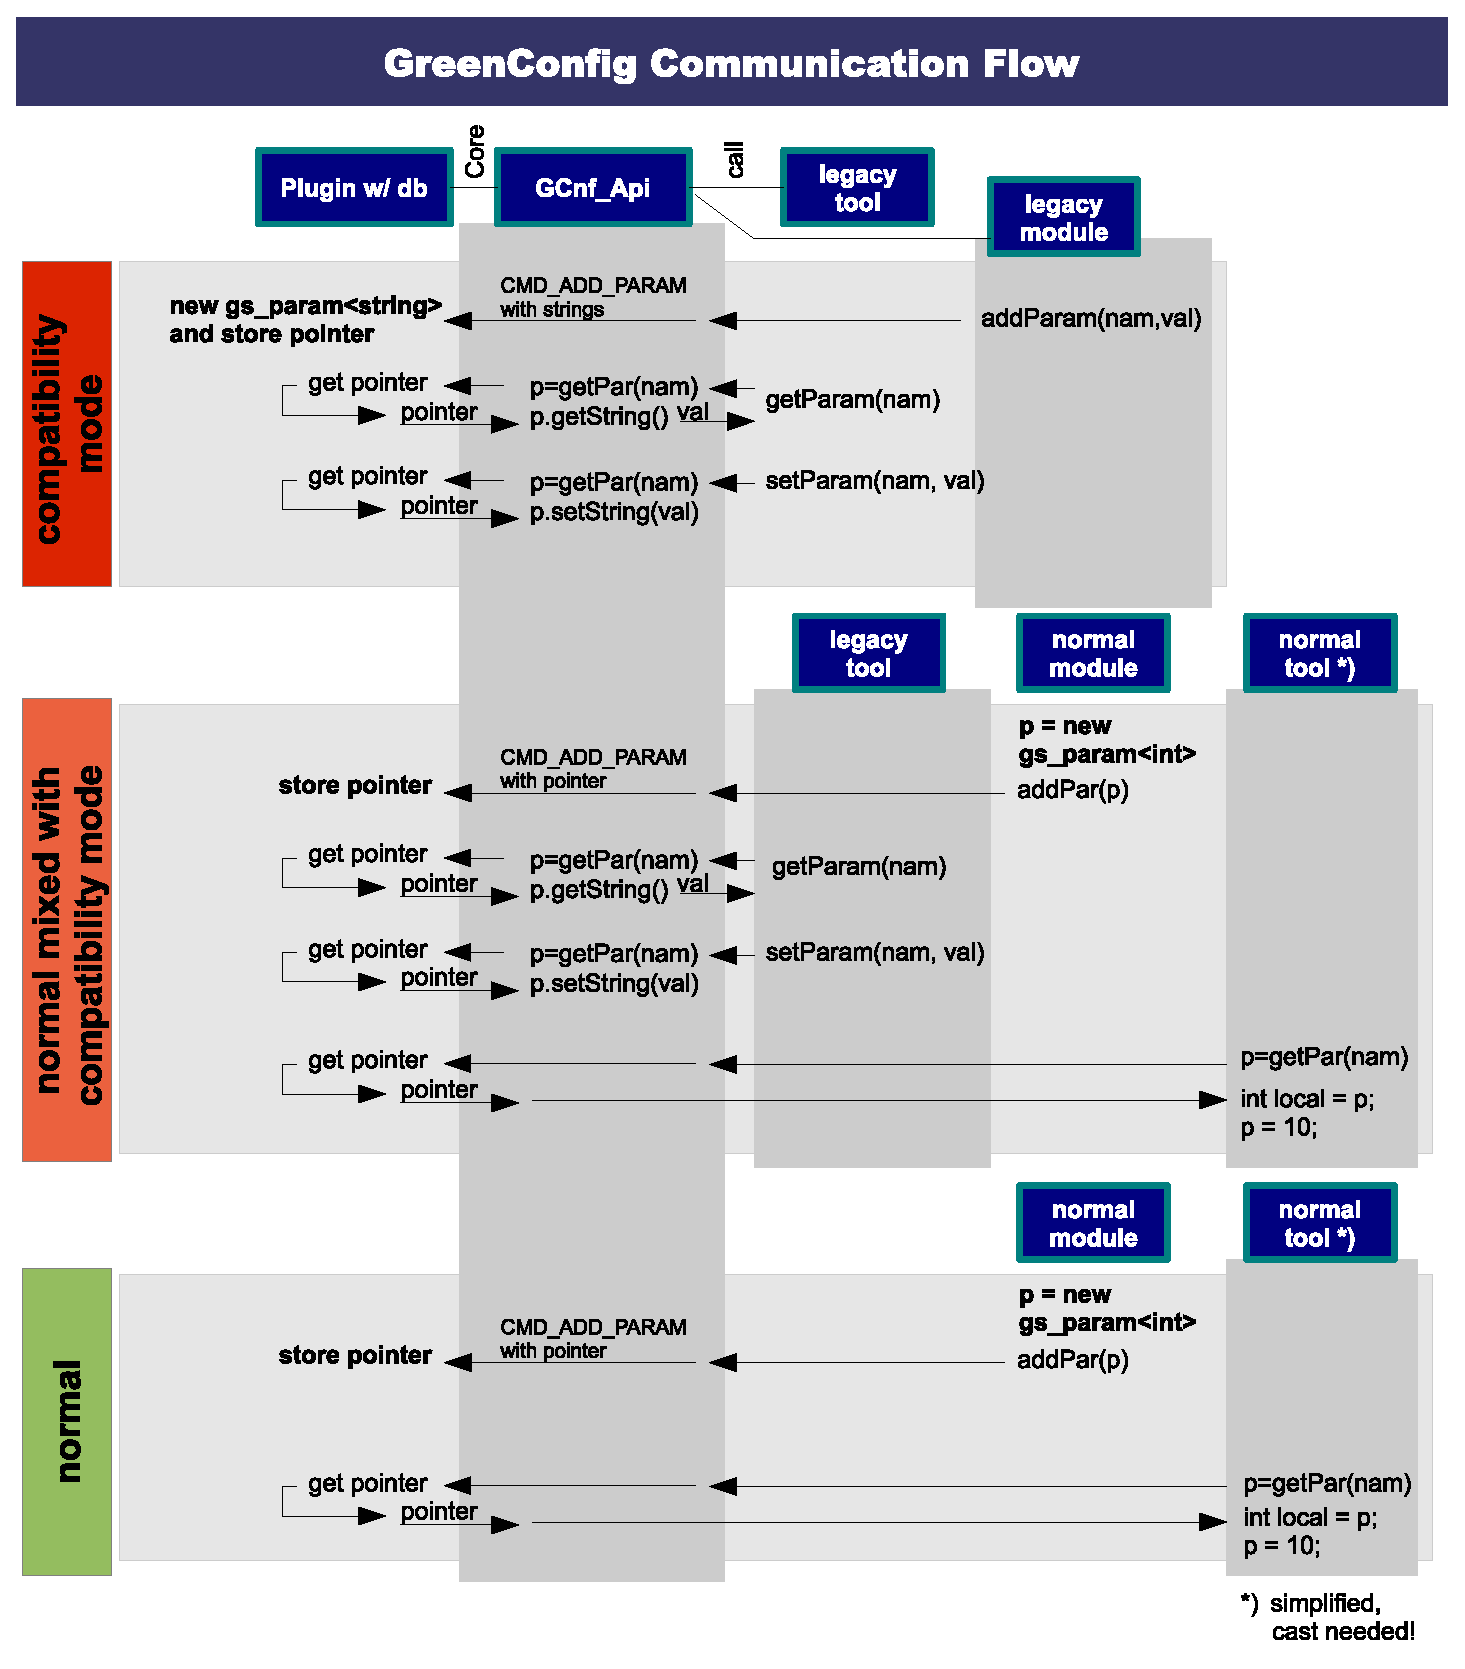
\includegraphics[width=\textwidth]{GreenConfig_Communication_Flow_normal.eps}}
	\caption{Three use cases with their GreenConfig communication and function call flow.}
	\label{fig:GCnfCommFlow}
\end{figure}


%%%%%%%%%%%%%%%%%%%%%%%%%%%%%%%
\section{Notes}
\begin{itemize}
	\item Parameter names may contain characters like variable names in C++ may (e.g. numbers, letters, underline character).
	\item Like XParam the \GreenConfig framework is able to parse command line parameters. We support a similar extensibility: user defined data types can be supported. They only have to be representable as string. The User API which uses these types has to convert between string and data type.
\end{itemize}


%%%%%%%%%%%%%%%%%%%%%%%%%%%%%%%
\section{Implementation code}
Visit the GreenSocs web page to get the newest revision of the \GreenConfig framework:\\
\href{http://drupal.greensocs.com/projects/GreenControl/GreenConfig}{http://drupal.greensocs.com/projects/GreenControl/GreenConfig}
